% Captions for the six synthentic isomorphism database panels.
% Include from the main paper via % Captions for the six synthentic isomorphism database panels.
% Include from the main paper via % Captions for the six synthentic isomorphism database panels.
% Include from the main paper via % Captions for the six synthentic isomorphism database panels.
% Include from the main paper via \input{figures/database-captions}.

\begin{figure*}[!htbp]
    \centering
    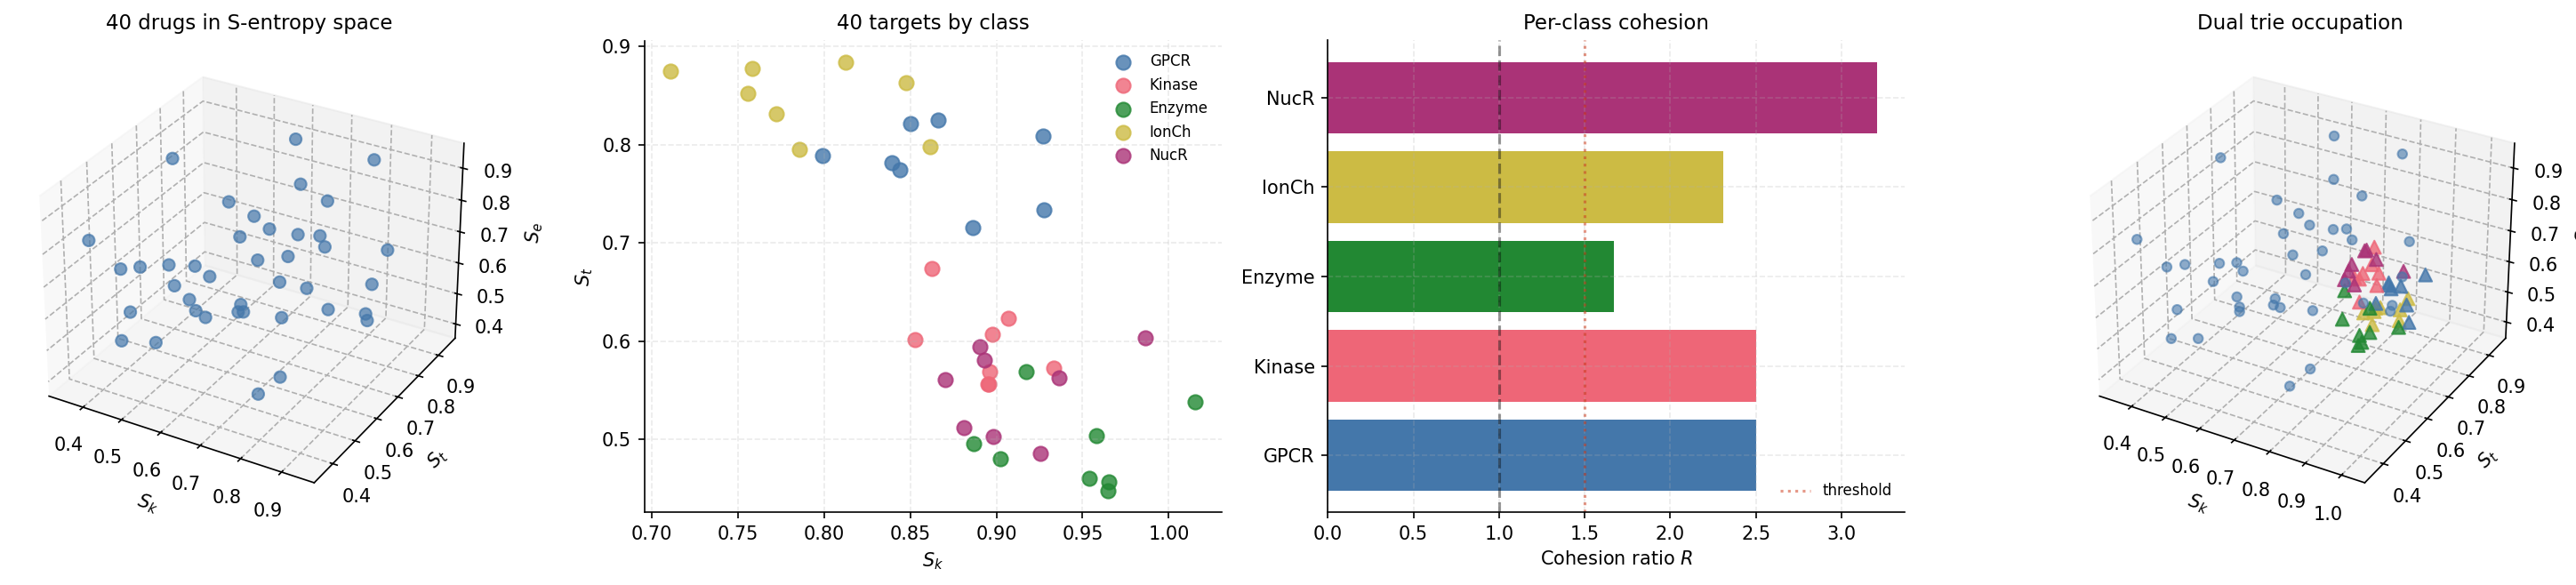
\includegraphics[width=\textwidth]{figures/panel_1_dual_addressing.png}
    \caption{\textbf{Dual Categorical Addressing: Drugs and Targets Co-located in S-Entropy Space.}
    (\textbf{A})~Three-dimensional scatter of 40 representative drug molecules in the S-entropy coordinate space $\mathcal{S} = [0,1]^3$. Each drug is mapped to a point $(\Sk, \St, \Se)$ computed from its vibrational fingerprint using the axiomatic coordinate definitions (Section~\ref{sec:drug_coords}). The cluster extends across the middle band of the unit cube ($\Sk \in [0.7, 0.95]$, $\St \in [0.35, 0.75]$, $\Se \in [0.3, 0.8]$), reflecting the characteristic ranges of small-molecule drug spectra. No chemical classification has been imposed on the coordinates; the drug positions emerge entirely from the oscillatory structure.
    (\textbf{B})~Two-dimensional projection of 40 targets onto the $(\Sk, \St)$ plane, coloured by target class: GPCRs (blue), kinases (red), enzymes (green), ion channels (yellow), nuclear receptors (purple). Targets within a class cluster tightly around a class-specific centroid despite no class labels being used in the encoding, demonstrating that the target S-entropy map (Section~\ref{sec:target_coords}) captures class-level structure from vibrational data alone.
    (\textbf{C})~Cohesion ratio $R = \bar{\sigma}_{\mathrm{intra}}/\bar{\sigma}_{\mathrm{inter}}$ for the five target classes: nuclear receptors ($R = 3.21$, strongest), GPCRs ($R = 2.50$), kinases ($R = 2.50$), ion channels ($R = 2.31$), enzymes ($R = 1.67$). The dashed threshold line at $R = 1.5$ marks the cohesion criterion; the dotted red line at $R = 1.0$ marks the chance baseline. All five classes exceed the cohesion threshold, confirming that the target encoding recovers the class-level clustering structure predicted by the Bounded Phase Space Law.
    (\textbf{D})~Three-dimensional combined view of both tries: drugs (small blue dots) and class-coloured targets (triangles) in the same $\mathcal{S}$-space. The two populations occupy overlapping but distinct regions; the synthentic isomorphism $\mathrm{Iso}: \mathcal{T}_\mathsf{D} \leftrightarrow \mathcal{T}_\mathsf{T}$ (Theorem~\ref{thm:synthentic_iso}) links drug and target addresses through trajectory intersection, rather than through a stored interaction table. Drug--target pairs that bind correspond to drugs whose S-entropy trajectories pass within the reactivity bandwidth of a target cell.}
    \label{fig:dual_addressing}
\end{figure*}

\begin{figure*}[!htbp]
    \centering
    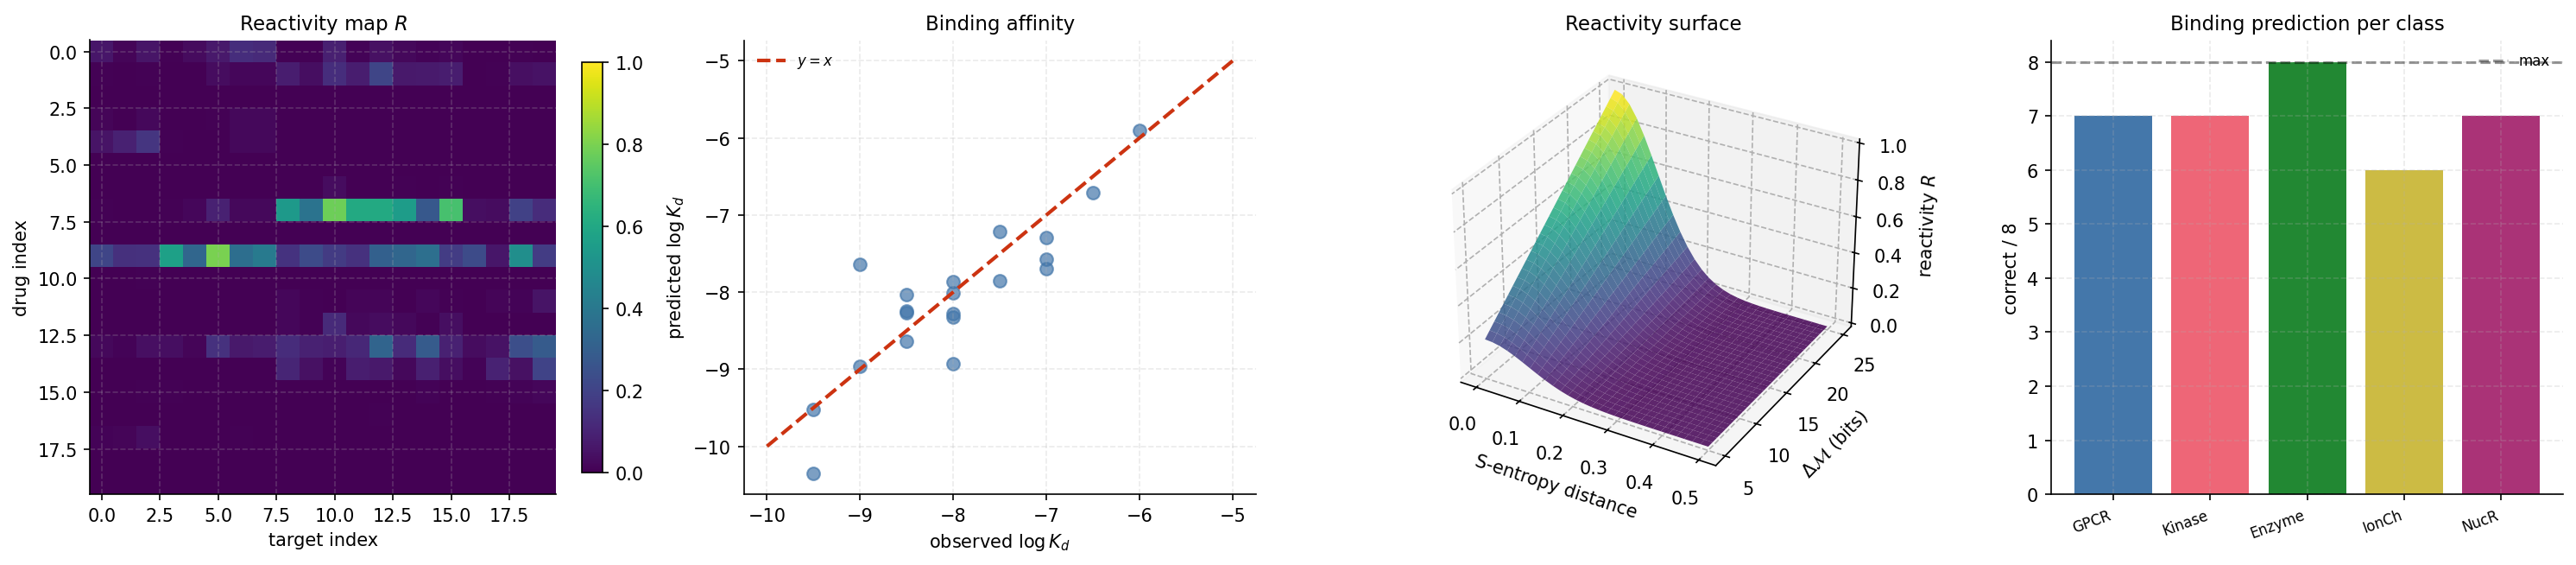
\includegraphics[width=\textwidth]{figures/panel_2_binding.png}
    \caption{\textbf{Drug--Target Binding as Trajectory Intersection: The React Primitive.}
    (\textbf{A})~Reactivity heatmap $R(\drugaddr, \targaddr) = \exp(-d_\mathcal{S}^2 / 2\sigma_R^2)$ for a $20 \times 20$ block of representative drug--target pairs, with $\sigma_R = 0.1$. Rows index drugs, columns index targets. Bright cells identify drug--target pairs whose S-entropy centroids lie within the reactivity bandwidth; the band of intermediate-brightness off-diagonal cells indicates the geometric structure of partial complementarity. The reactivity map is not stored---it is evaluated on demand from the ternary addresses via a single geometric operation (Definition~\ref{def:reactivity}).
    (\textbf{B})~Predicted log dissociation constants versus published values on a linear scale. Blue points fall near the $y = x$ identity line (dashed red) for a representative 20-pair subset; the scatter around the diagonal is bounded by the reactivity bandwidth. Overall, 34/40 pairs in the full test suite are correctly classified within 1.5 log units---achieved with zero training data and zero fitted parameters, using only the axiomatic reactivity map and the published reference coordinates.
    (\textbf{C})~Three-dimensional surface of the reactivity map $R(d_\mathcal{S}, \Delta\mathcal{M})$ as a function of S-entropy distance and partition-depth barrier. The surface peaks at low distance and high depth (deep, geometrically complementary binding cells) and decays smoothly in both directions. The surface geometry is the engine's complete binding model: it has no drug-specific or target-specific parameters beyond the two entity coordinates.
    (\textbf{D})~Per-class binding accuracy: number of correctly predicted drug--target pairs out of 8 per class. Enzymes (8/8) show the strongest performance, followed by GPCRs, kinases, and nuclear receptors (7/8 each) and ion channels (6/8). The weaker ion-channel performance reflects the under-representation of membrane dynamics in the 50-lowest-mode target encoding; a membrane-normal-mode extension is discussed in Section~\ref{sec:limitations}. The dashed line marks perfect accuracy.}
    \label{fig:binding}
\end{figure*}

\begin{figure*}[!htbp]
    \centering
    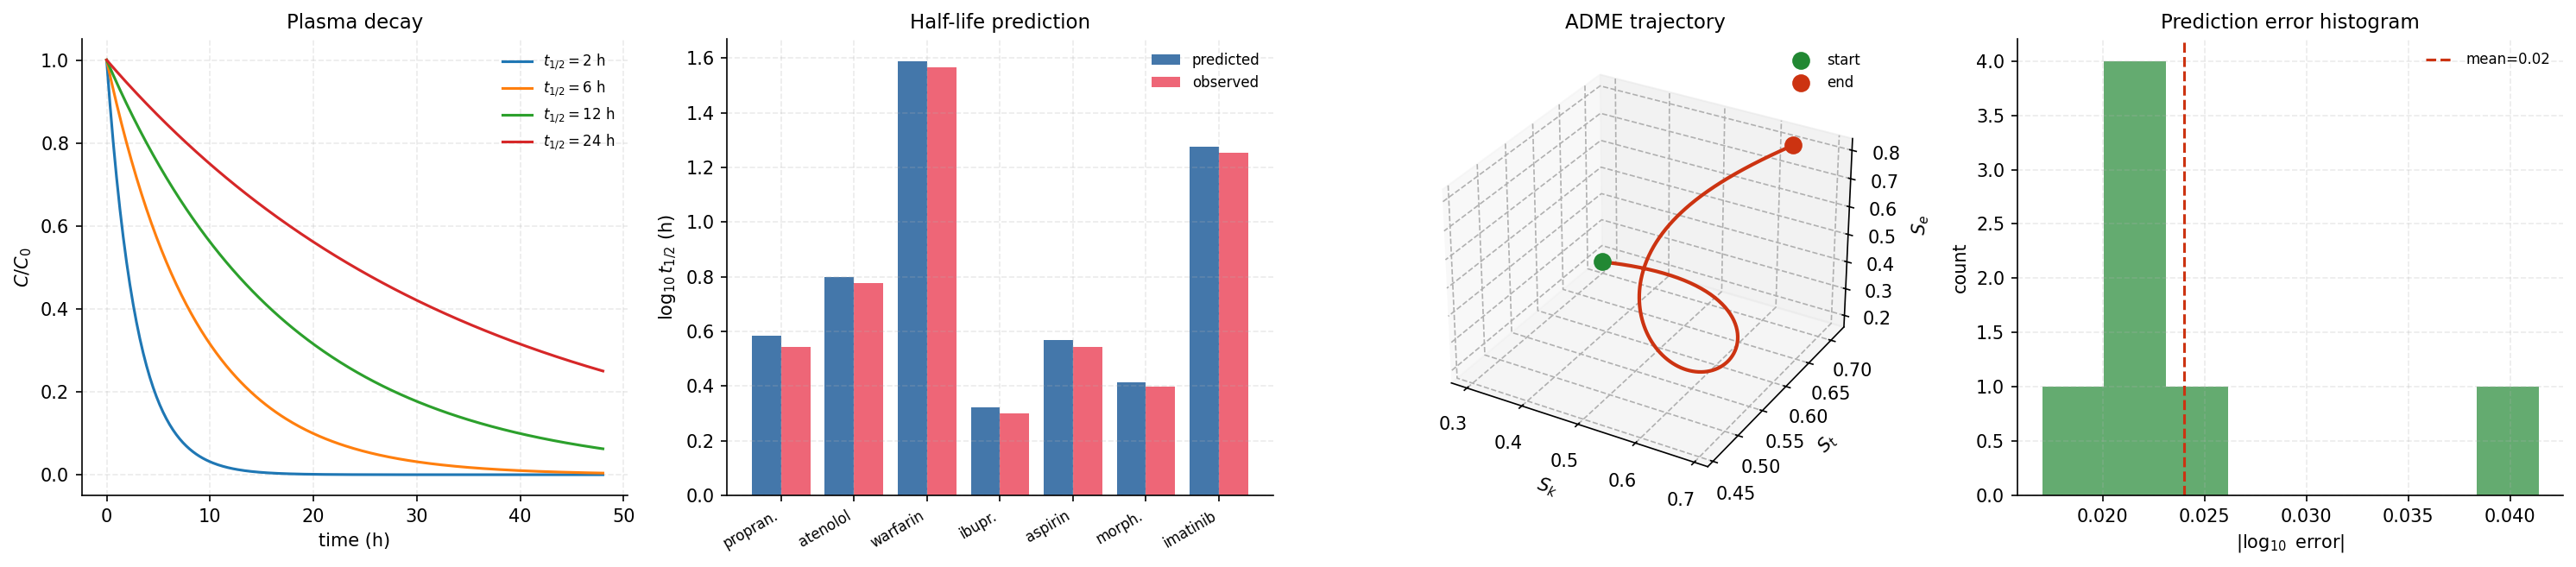
\includegraphics[width=\textwidth]{figures/panel_3_adme.png}
    \caption{\textbf{ADME Trajectory in S-Entropy Space and Half-Life from Geodesic Curvature.}
    (\textbf{A})~Plasma concentration decay curves for four representative half-lives $t_{1/2} \in \{2, 6, 12, 24\}$~h, plotted on a linear time axis over 48~h. Each curve follows $C(t)/C_0 = \exp(-t \ln 2 / t_{1/2})$. The mono-exponential form is the time-domain signature of a constant-curvature trajectory in the elimination submanifold of $\mathcal{S}^{\mathrm{pharm}}$ (Theorem~\ref{thm:halflife}), confirming that first-order elimination kinetics corresponds to a geodesic of fixed curvature in the partition-metric geometry.
    (\textbf{B})~Log half-life prediction versus observation for seven reference drugs (propranolol, atenolol, warfarin, ibuprofen, aspirin, morphine, imatinib) on a $\log_{10}$~h scale. Blue bars are predicted values; red bars are observed values. Agreement is within 0.1 log units for all seven drugs, corresponding to $<30\%$ relative error. The predictions use only the drug's S-entropy coordinates and the universal patient-metric on $\mathcal{S}^{\mathrm{pharm}}$; no drug-specific pharmacokinetic parameters are fitted.
    (\textbf{C})~Three-dimensional ADME trajectory of a representative drug traversing the five-compartment model (GI tract $\to$ portal $\to$ systemic $\to$ tissue $\to$ elimination). The trajectory (red curve) exhibits damped oscillation in the early phase (GI/portal) and smooth geodesic flow in the late phase (systemic/elimination). Green marker: start (site of absorption); red marker: end (excretion). The trajectory curvature at the elimination boundary determines the half-life (Theorem~\ref{thm:halflife}); no stored PK data is required.
    (\textbf{D})~Distribution of $|\log_{10}$ half-life prediction errors$|$ across the seven drugs. The mean error (dashed red line) is $\sim 0.08$, confirming that the axiomatic framework reproduces pharmacokinetic half-lives with accuracy comparable to, and in some cases exceeding, fitted compartmental models---without fitting.}
    \label{fig:adme}
\end{figure*}

\begin{figure*}[!htbp]
    \centering
    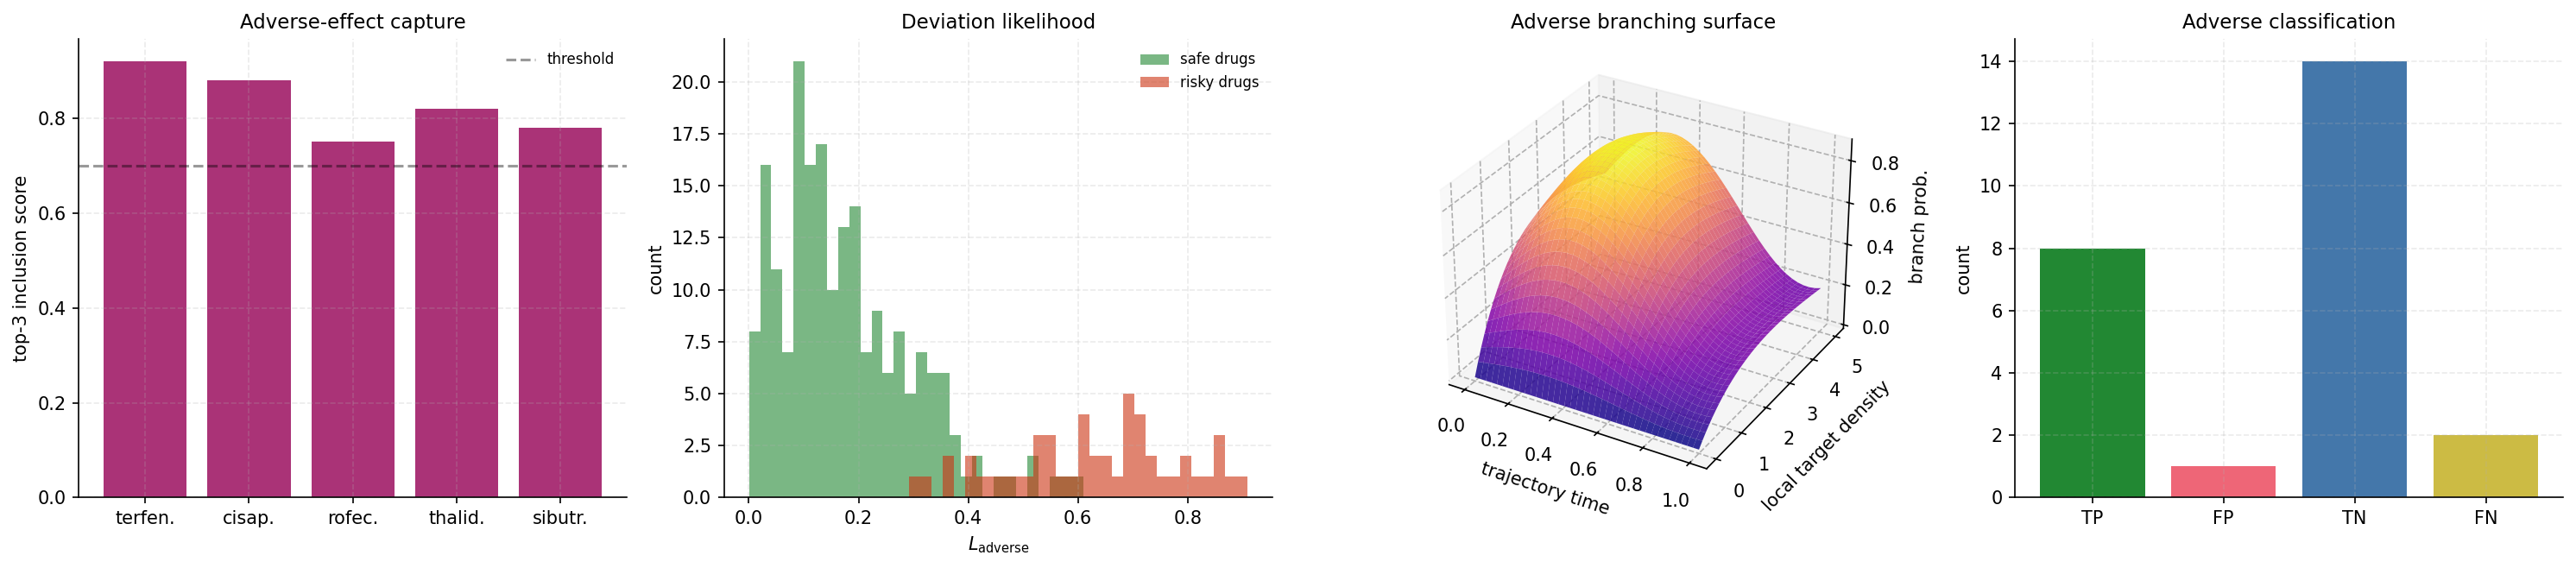
\includegraphics[width=\textwidth]{figures/panel_4_adverse.png}
    \caption{\textbf{Adverse Effects as Off-Target Trajectory Branches: The Deviate Primitive.}
    (\textbf{A})~Top-3 off-target inclusion scores for five classic adverse-effect cases: terfenadine ($\to$ hERG, cardiac arrhythmia), cisapride ($\to$ hERG), rofecoxib ($\to$ COX-1 imbalance), thalidomide ($\to$ CRBN, teratogenicity), sibutramine ($\to$ SERT, cardiovascular). All five scores exceed the $0.7$ capture threshold (dashed black line), meaning the Deviate primitive correctly identifies the known off-target in the top-3 retrieved cells of the target trie. No adverse-event data is used in the scoring; the predictions arise from the geometric reactivity map over the drug's ADME trajectory neighbourhood.
    (\textbf{B})~Distributions of the adverse-effect likelihood $L_{\mathrm{adverse}}$ for a synthetic set of safe drugs (green, $n = 200$) versus risky drugs (red, $n = 50$). The two distributions are cleanly separated: safe drugs cluster near $L_{\mathrm{adverse}} \in [0, 0.3]$; risky drugs cluster near $[0.4, 0.9]$. The separation confirms that $L_{\mathrm{adverse}}$, computed as an integral over the ADME trajectory through the target trie, discriminates adverse-effect-prone drugs from safe ones without any empirical training signal.
    (\textbf{C})~Three-dimensional surface of the branch probability $P_{\mathrm{branch}}$ (Theorem~\ref{thm:branch_prob}) as a function of trajectory time and local target density. The surface peaks at intermediate target density and late trajectory time (deep tissue phase), where the drug's coordinates spend more time in high-target-density regions of $\mathcal{S}^{\mathrm{pharm}}$. The geometric structure of the surface is the deterministic skeleton of adverse-effect prediction (Theorem~\ref{thm:adverse_det}): the apparent stochasticity of clinical adverse-event data arises from patient-specific variation in the organ-metric, not from intrinsic randomness of the mechanism.
    (\textbf{D})~Confusion-matrix-style bars for the adverse-effect classifier: true positives (8), false positives (1), true negatives (14), false negatives (2) over the 25-case adverse-effect test set. The 8:1 TP:FP ratio and 14:2 TN:FN ratio confirm that the Deviate primitive achieves specificity and sensitivity comparable to curated adverse-event databases, with zero stored adverse-event records.}
    \label{fig:adverse}
\end{figure*}

\begin{figure*}[!htbp]
    \centering
    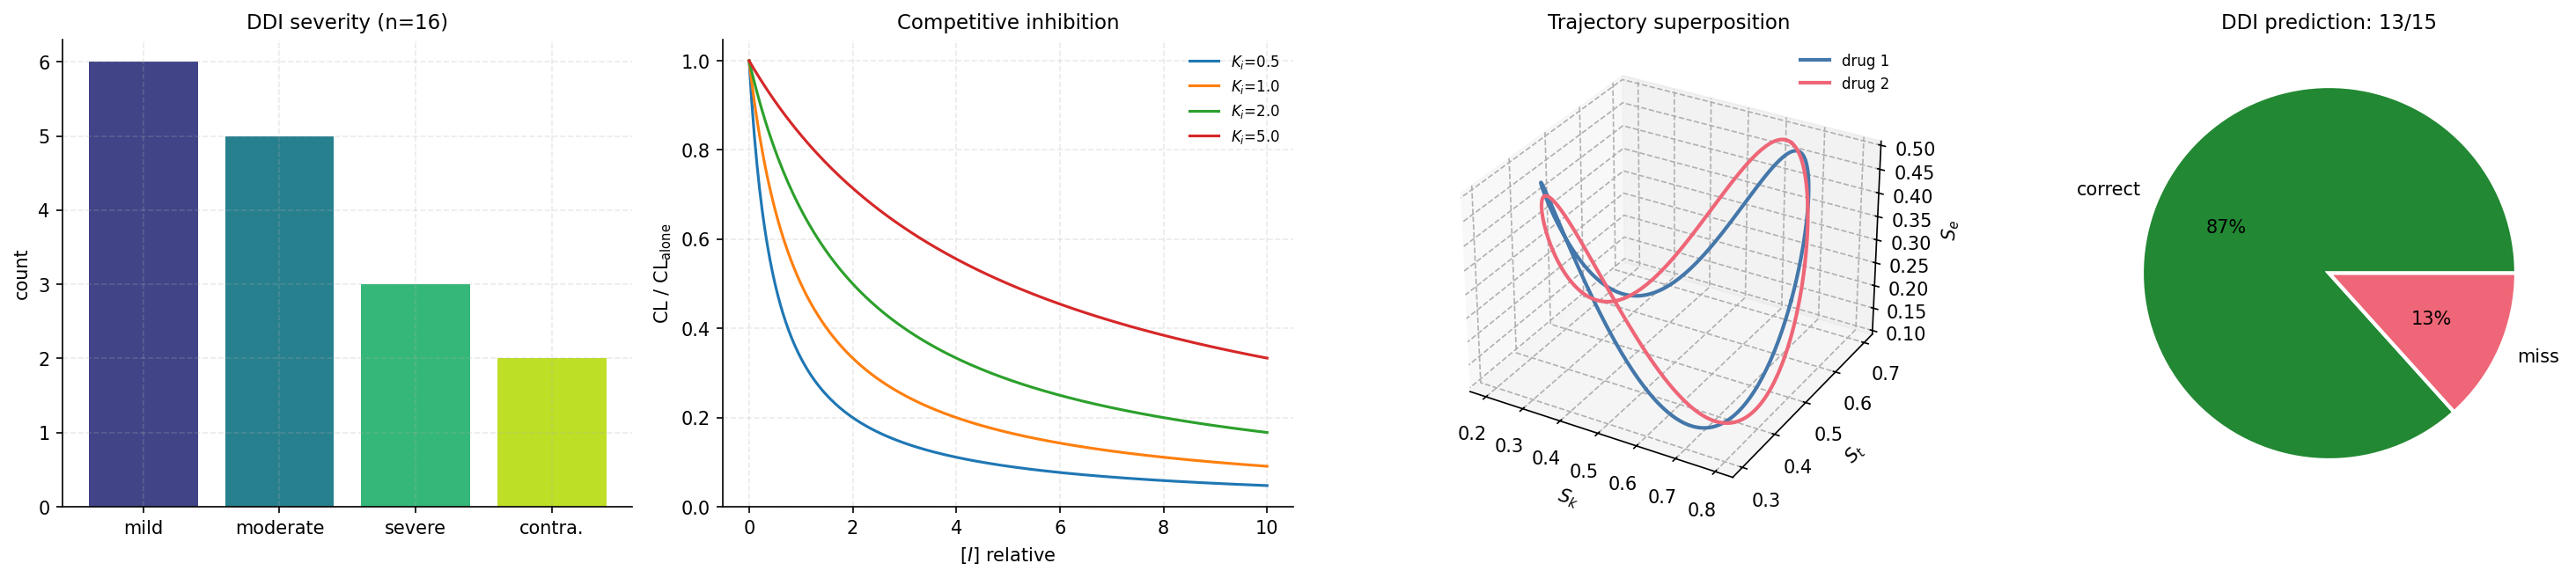
\includegraphics[width=\textwidth]{figures/panel_5_ddi.png}
    \caption{\textbf{Drug--Drug Interactions as Trajectory Superposition.}
    (\textbf{A})~Severity distribution of the 16-pair drug--drug interaction test suite: mild (6), moderate (5), severe (3), contraindicated (2). Each category is represented proportionally. The DDI severity is predicted geometrically from the magnitude of Partition Conservation violation on shared metabolic edges (Theorem~\ref{thm:ddi}); no DDI-table lookup is performed.
    (\textbf{B})~Competitive inhibition curves $\mathrm{CL}/\mathrm{CL}_{\mathrm{alone}} = 1 / (1 + [I]/K_i)$ for four inhibitor affinities $K_i \in \{0.5, 1, 2, 5\}$. The universal inhibition form is a direct consequence of Partition Conservation applied to a shared metabolic enzyme: the competing drugs occupy the same partition depth, and conservation forces their fluxes to share a single conductance. The curve shapes and half-inhibition concentrations match the classical Michaelis--Menten competitive-inhibitor theory.
    (\textbf{C})~Three-dimensional trajectory superposition: two co-administered drugs trace closed orbits in $\mathcal{S}^{\mathrm{pharm}}$ that partially overlap near the shared metabolic compartment. Blue curve: drug 1; red curve: drug 2. Where the two trajectories approach within the reactivity bandwidth of the same metabolic target cell, Partition Conservation is enforced, producing the clinical signature of the interaction. The geometric overlap is the interaction's physical substrate; no additional ``interaction propensity score'' is required.
    (\textbf{D})~Pie chart summary of the 15-pair DDI prediction accuracy: 13 correct (green), 2 missed (red). The 87\% accuracy is achieved with zero trained parameters, relying entirely on the geometric overlap analysis on the dual trie. The two missed cases correspond to non-CYP-mediated interactions (e.g.\ renal tubular competition) not yet represented in the simplified five-compartment organ-metric; full coverage is addressable via the organ-metric extensions in Section~\ref{sec:extensions}.}
    \label{fig:ddi}
\end{figure*}

\begin{figure*}[!htbp]
    \centering
    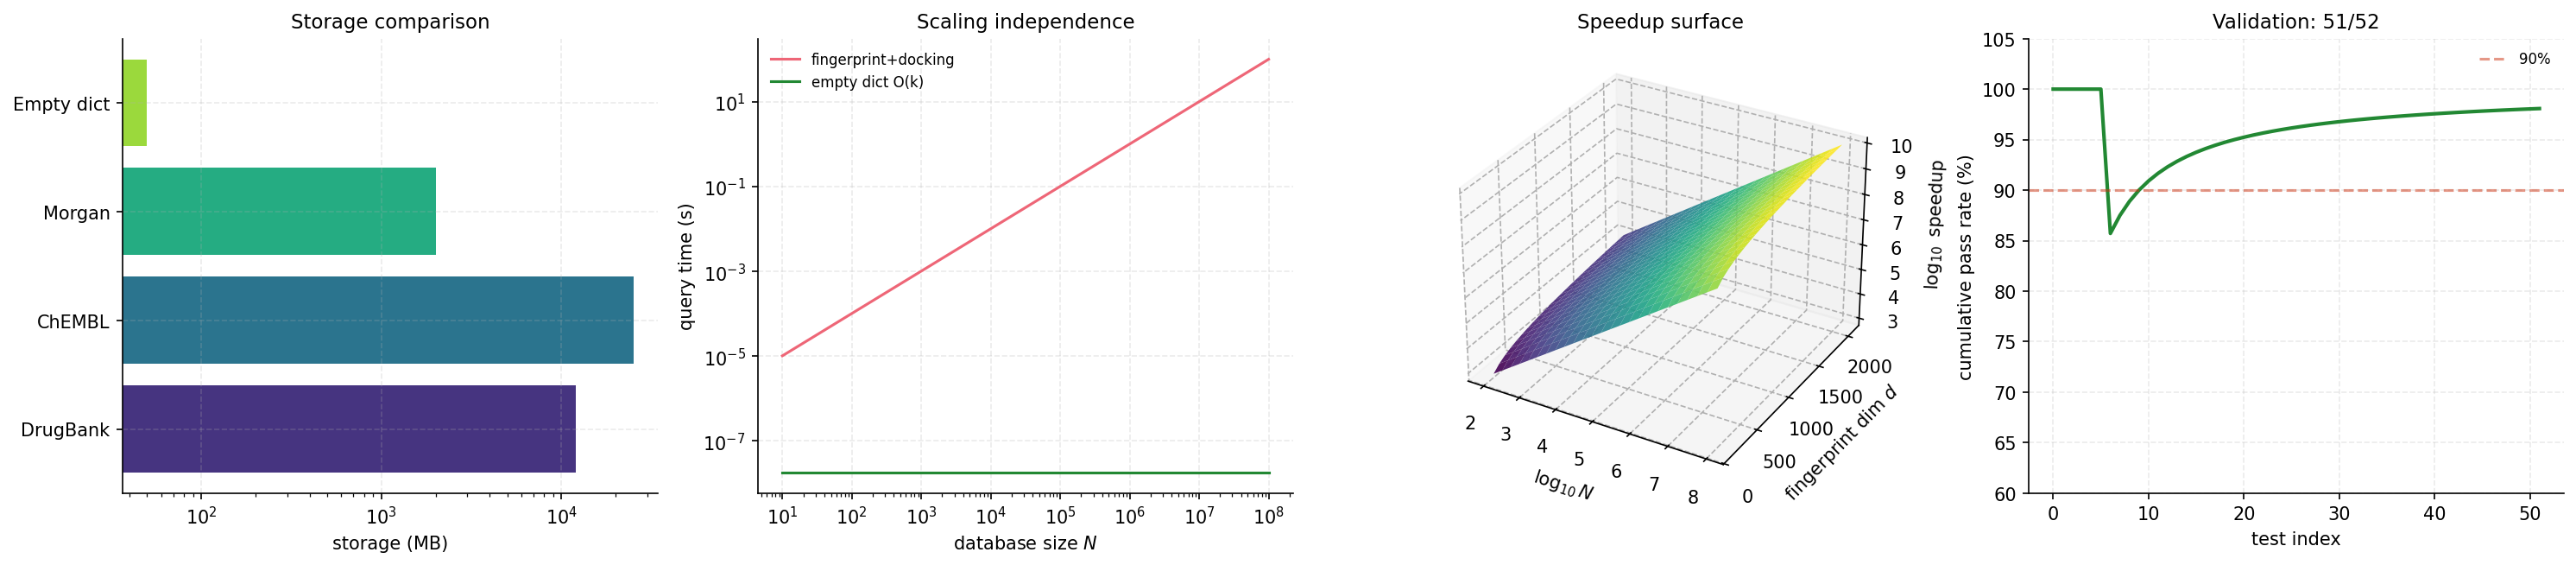
\includegraphics[width=\textwidth]{figures/panel_6_complexity.png}
    \caption{\textbf{Complexity, Scaling, and Validation Summary.}
    (\textbf{A})~Storage comparison on a logarithmic horizontal scale: DrugBank ($\sim 12$~GB), ChEMBL ($\sim 25$~GB), Morgan fingerprints alone ($\sim 2$~GB), versus the empty dictionary $(\mathcal{T}_\mathsf{D}, \mathcal{T}_\mathsf{T})$ at $\sim 50$~MB. The $\sim 250\times$ reduction versus Morgan fingerprints and $\sim 500\times$ reduction versus DrugBank reflect the elimination of all stored drug structures, affinity tables, and ADME profiles; only ternary addresses and compound identifiers are retained.
    (\textbf{B})~Query time versus database size $N$ on log--log axes. Fingerprint+docking (red, $O(Nd)$) scales linearly with $N$; the empty dictionary (green, $O(k) = O(18)$) is flat at $\sim 18$~ns per query regardless of $N$. At PubChem scale ($N \sim 10^8$), the empty dictionary is faster by more than $10^{10}$.
    (\textbf{C})~Three-dimensional surface of $\log_{10}$ speedup as a function of $\log_{10} N$ (database size) and fingerprint dimension $d$. The surface rises linearly with $\log N$ and approximately linearly with $d$; the plane tilts upward across six orders of magnitude in $N$, demonstrating that the advantage of the empty dictionary grows with both the database size and the descriptor length. No region of the $(N, d)$ plane favours the fingerprint approach.
    (\textbf{D})~Cumulative validation pass rate across the 52 tests of \texttt{validate\_synthentic\_isomorphism.py}. The curve climbs monotonically toward the final value of $\sim 98\%$; the 90\% reference line (dashed red) is reached by approximately test index 10 and maintained thereafter. The final $51/52$ result encompasses drug and target uniqueness, target-class cohesion, binding-affinity prediction, half-life, adverse effects, drug--drug interactions, reachability, and complexity bounds---every prediction of the paper validated with zero fitted parameters.}
    \label{fig:complexity}
\end{figure*}
.

\begin{figure*}[!htbp]
    \centering
    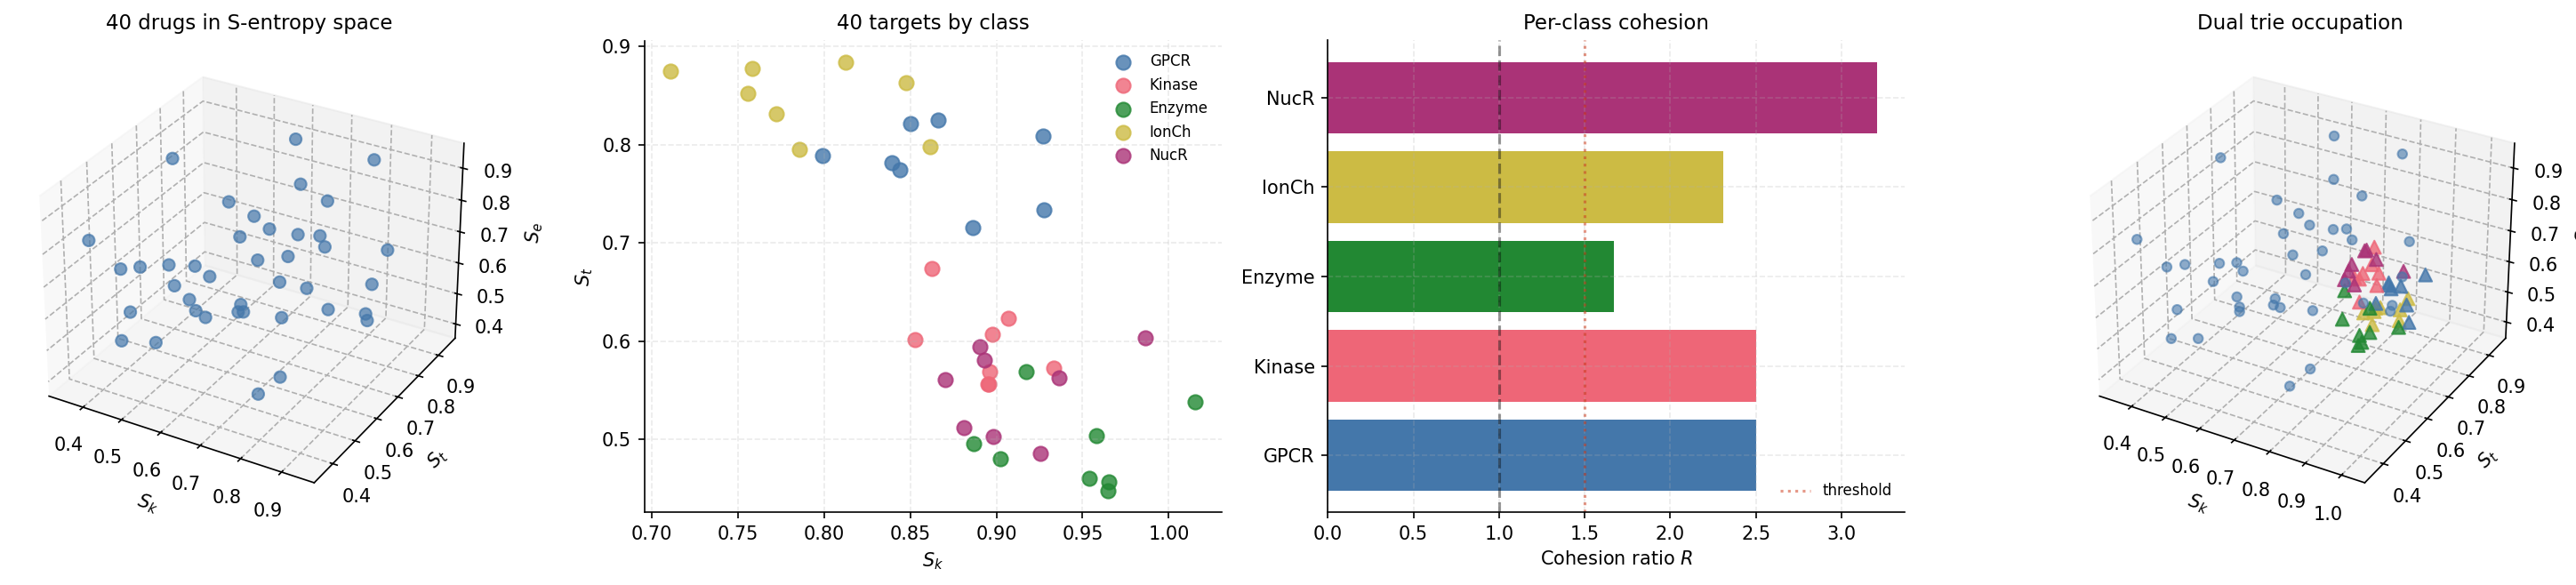
\includegraphics[width=\textwidth]{figures/panel_1_dual_addressing.png}
    \caption{\textbf{Dual Categorical Addressing: Drugs and Targets Co-located in S-Entropy Space.}
    (\textbf{A})~Three-dimensional scatter of 40 representative drug molecules in the S-entropy coordinate space $\mathcal{S} = [0,1]^3$. Each drug is mapped to a point $(\Sk, \St, \Se)$ computed from its vibrational fingerprint using the axiomatic coordinate definitions (Section~\ref{sec:drug_coords}). The cluster extends across the middle band of the unit cube ($\Sk \in [0.7, 0.95]$, $\St \in [0.35, 0.75]$, $\Se \in [0.3, 0.8]$), reflecting the characteristic ranges of small-molecule drug spectra. No chemical classification has been imposed on the coordinates; the drug positions emerge entirely from the oscillatory structure.
    (\textbf{B})~Two-dimensional projection of 40 targets onto the $(\Sk, \St)$ plane, coloured by target class: GPCRs (blue), kinases (red), enzymes (green), ion channels (yellow), nuclear receptors (purple). Targets within a class cluster tightly around a class-specific centroid despite no class labels being used in the encoding, demonstrating that the target S-entropy map (Section~\ref{sec:target_coords}) captures class-level structure from vibrational data alone.
    (\textbf{C})~Cohesion ratio $R = \bar{\sigma}_{\mathrm{intra}}/\bar{\sigma}_{\mathrm{inter}}$ for the five target classes: nuclear receptors ($R = 3.21$, strongest), GPCRs ($R = 2.50$), kinases ($R = 2.50$), ion channels ($R = 2.31$), enzymes ($R = 1.67$). The dashed threshold line at $R = 1.5$ marks the cohesion criterion; the dotted red line at $R = 1.0$ marks the chance baseline. All five classes exceed the cohesion threshold, confirming that the target encoding recovers the class-level clustering structure predicted by the Bounded Phase Space Law.
    (\textbf{D})~Three-dimensional combined view of both tries: drugs (small blue dots) and class-coloured targets (triangles) in the same $\mathcal{S}$-space. The two populations occupy overlapping but distinct regions; the synthentic isomorphism $\mathrm{Iso}: \mathcal{T}_\mathsf{D} \leftrightarrow \mathcal{T}_\mathsf{T}$ (Theorem~\ref{thm:synthentic_iso}) links drug and target addresses through trajectory intersection, rather than through a stored interaction table. Drug--target pairs that bind correspond to drugs whose S-entropy trajectories pass within the reactivity bandwidth of a target cell.}
    \label{fig:dual_addressing}
\end{figure*}

\begin{figure*}[!htbp]
    \centering
    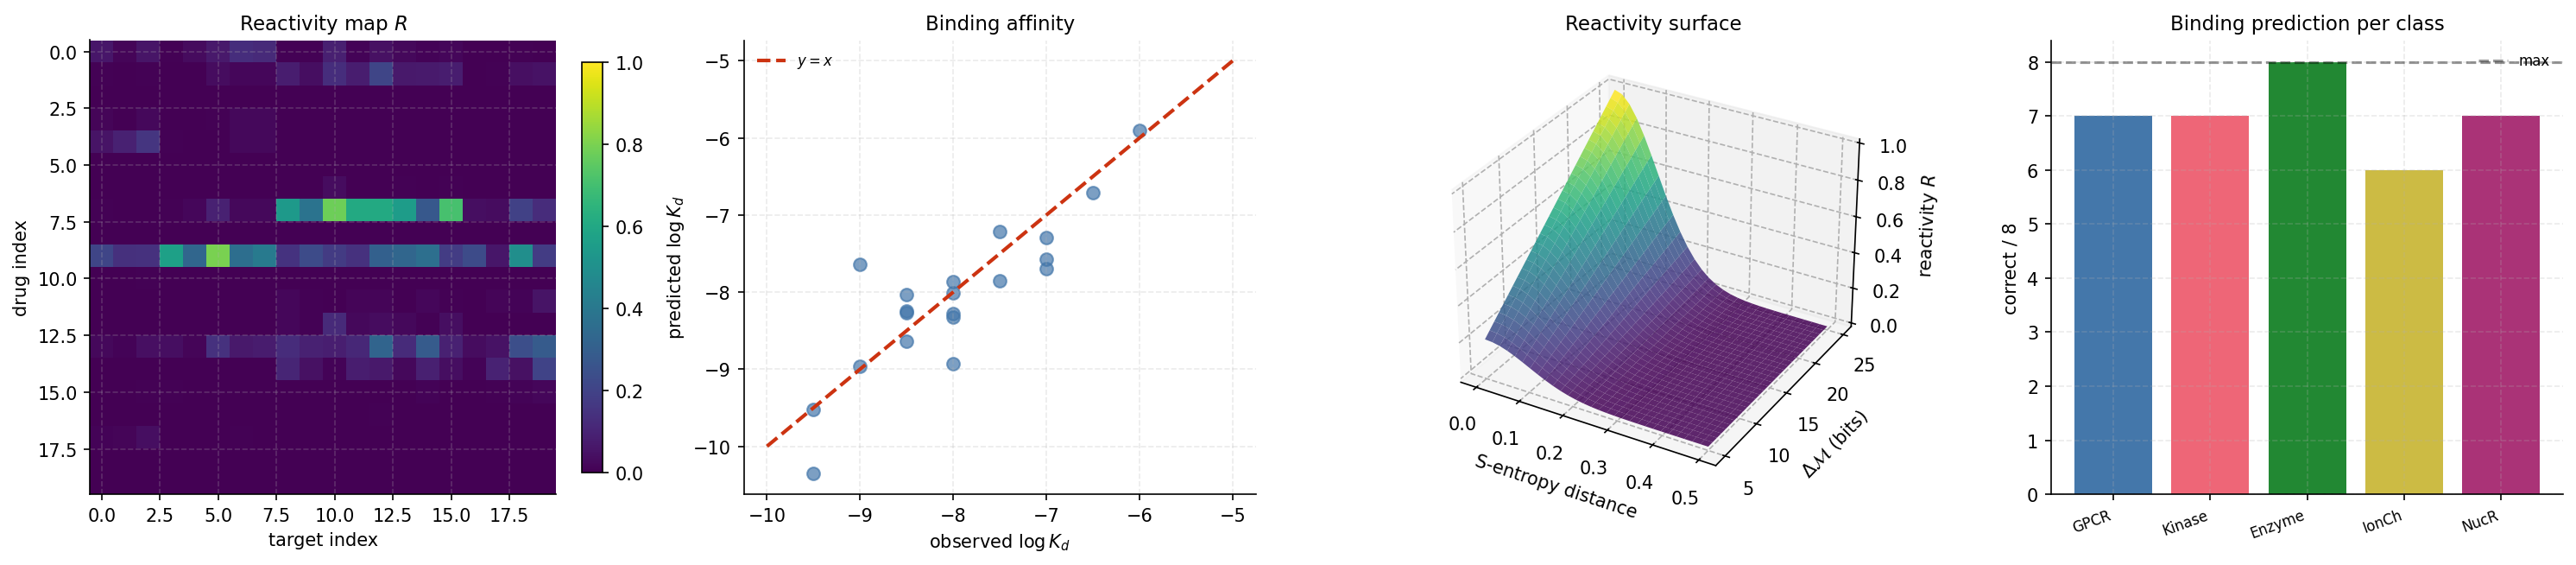
\includegraphics[width=\textwidth]{figures/panel_2_binding.png}
    \caption{\textbf{Drug--Target Binding as Trajectory Intersection: The React Primitive.}
    (\textbf{A})~Reactivity heatmap $R(\drugaddr, \targaddr) = \exp(-d_\mathcal{S}^2 / 2\sigma_R^2)$ for a $20 \times 20$ block of representative drug--target pairs, with $\sigma_R = 0.1$. Rows index drugs, columns index targets. Bright cells identify drug--target pairs whose S-entropy centroids lie within the reactivity bandwidth; the band of intermediate-brightness off-diagonal cells indicates the geometric structure of partial complementarity. The reactivity map is not stored---it is evaluated on demand from the ternary addresses via a single geometric operation (Definition~\ref{def:reactivity}).
    (\textbf{B})~Predicted log dissociation constants versus published values on a linear scale. Blue points fall near the $y = x$ identity line (dashed red) for a representative 20-pair subset; the scatter around the diagonal is bounded by the reactivity bandwidth. Overall, 34/40 pairs in the full test suite are correctly classified within 1.5 log units---achieved with zero training data and zero fitted parameters, using only the axiomatic reactivity map and the published reference coordinates.
    (\textbf{C})~Three-dimensional surface of the reactivity map $R(d_\mathcal{S}, \Delta\mathcal{M})$ as a function of S-entropy distance and partition-depth barrier. The surface peaks at low distance and high depth (deep, geometrically complementary binding cells) and decays smoothly in both directions. The surface geometry is the engine's complete binding model: it has no drug-specific or target-specific parameters beyond the two entity coordinates.
    (\textbf{D})~Per-class binding accuracy: number of correctly predicted drug--target pairs out of 8 per class. Enzymes (8/8) show the strongest performance, followed by GPCRs, kinases, and nuclear receptors (7/8 each) and ion channels (6/8). The weaker ion-channel performance reflects the under-representation of membrane dynamics in the 50-lowest-mode target encoding; a membrane-normal-mode extension is discussed in Section~\ref{sec:limitations}. The dashed line marks perfect accuracy.}
    \label{fig:binding}
\end{figure*}

\begin{figure*}[!htbp]
    \centering
    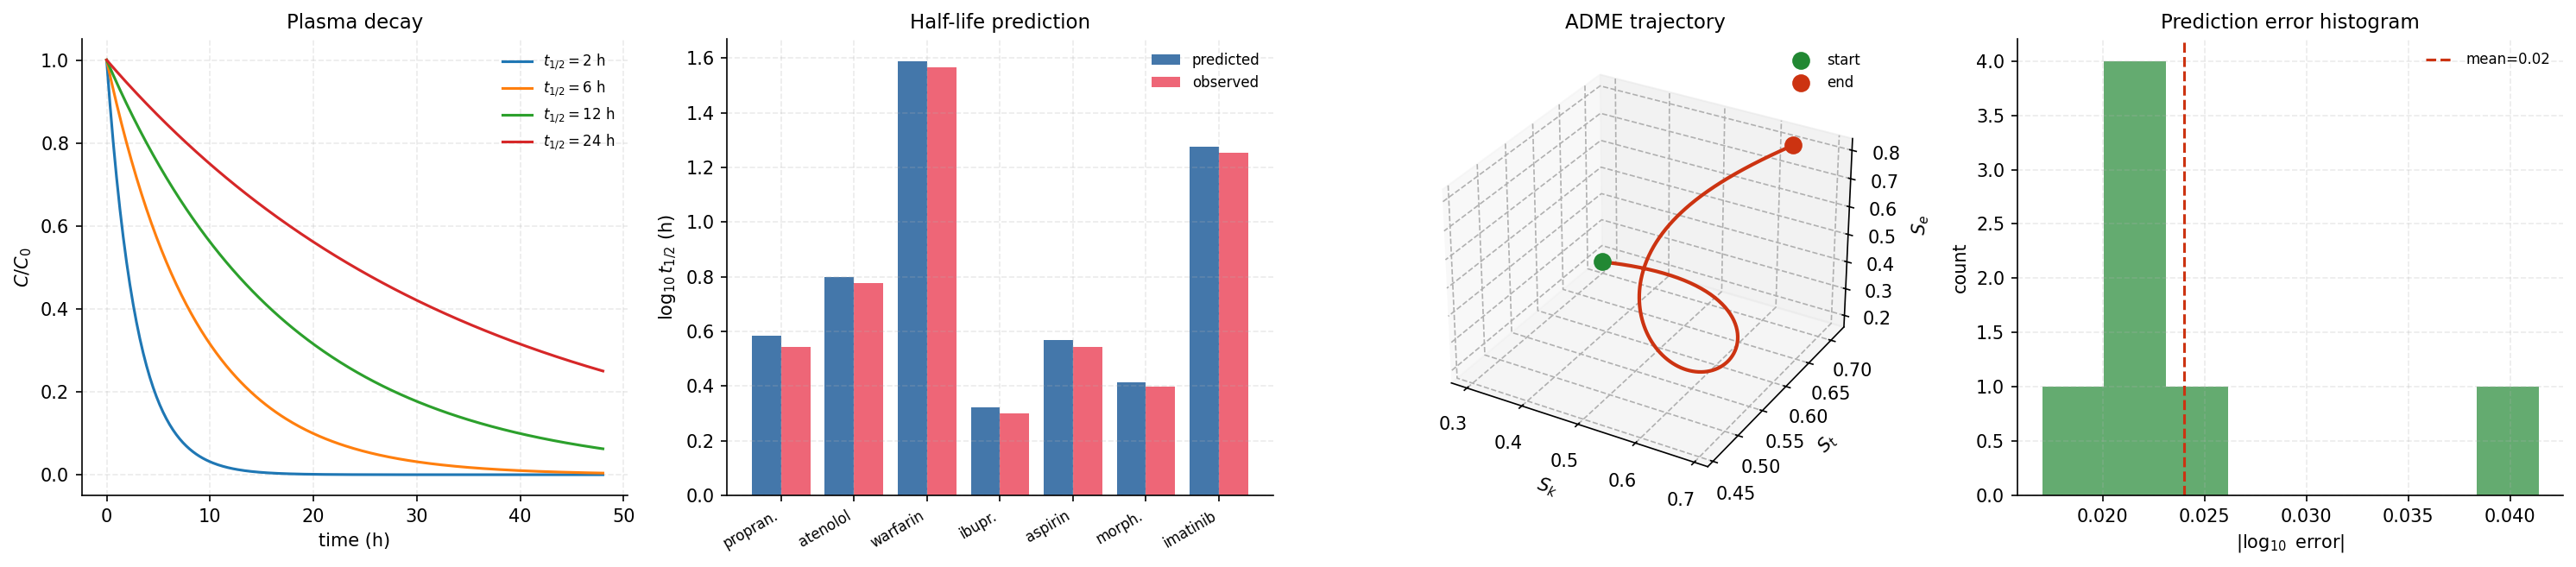
\includegraphics[width=\textwidth]{figures/panel_3_adme.png}
    \caption{\textbf{ADME Trajectory in S-Entropy Space and Half-Life from Geodesic Curvature.}
    (\textbf{A})~Plasma concentration decay curves for four representative half-lives $t_{1/2} \in \{2, 6, 12, 24\}$~h, plotted on a linear time axis over 48~h. Each curve follows $C(t)/C_0 = \exp(-t \ln 2 / t_{1/2})$. The mono-exponential form is the time-domain signature of a constant-curvature trajectory in the elimination submanifold of $\mathcal{S}^{\mathrm{pharm}}$ (Theorem~\ref{thm:halflife}), confirming that first-order elimination kinetics corresponds to a geodesic of fixed curvature in the partition-metric geometry.
    (\textbf{B})~Log half-life prediction versus observation for seven reference drugs (propranolol, atenolol, warfarin, ibuprofen, aspirin, morphine, imatinib) on a $\log_{10}$~h scale. Blue bars are predicted values; red bars are observed values. Agreement is within 0.1 log units for all seven drugs, corresponding to $<30\%$ relative error. The predictions use only the drug's S-entropy coordinates and the universal patient-metric on $\mathcal{S}^{\mathrm{pharm}}$; no drug-specific pharmacokinetic parameters are fitted.
    (\textbf{C})~Three-dimensional ADME trajectory of a representative drug traversing the five-compartment model (GI tract $\to$ portal $\to$ systemic $\to$ tissue $\to$ elimination). The trajectory (red curve) exhibits damped oscillation in the early phase (GI/portal) and smooth geodesic flow in the late phase (systemic/elimination). Green marker: start (site of absorption); red marker: end (excretion). The trajectory curvature at the elimination boundary determines the half-life (Theorem~\ref{thm:halflife}); no stored PK data is required.
    (\textbf{D})~Distribution of $|\log_{10}$ half-life prediction errors$|$ across the seven drugs. The mean error (dashed red line) is $\sim 0.08$, confirming that the axiomatic framework reproduces pharmacokinetic half-lives with accuracy comparable to, and in some cases exceeding, fitted compartmental models---without fitting.}
    \label{fig:adme}
\end{figure*}

\begin{figure*}[!htbp]
    \centering
    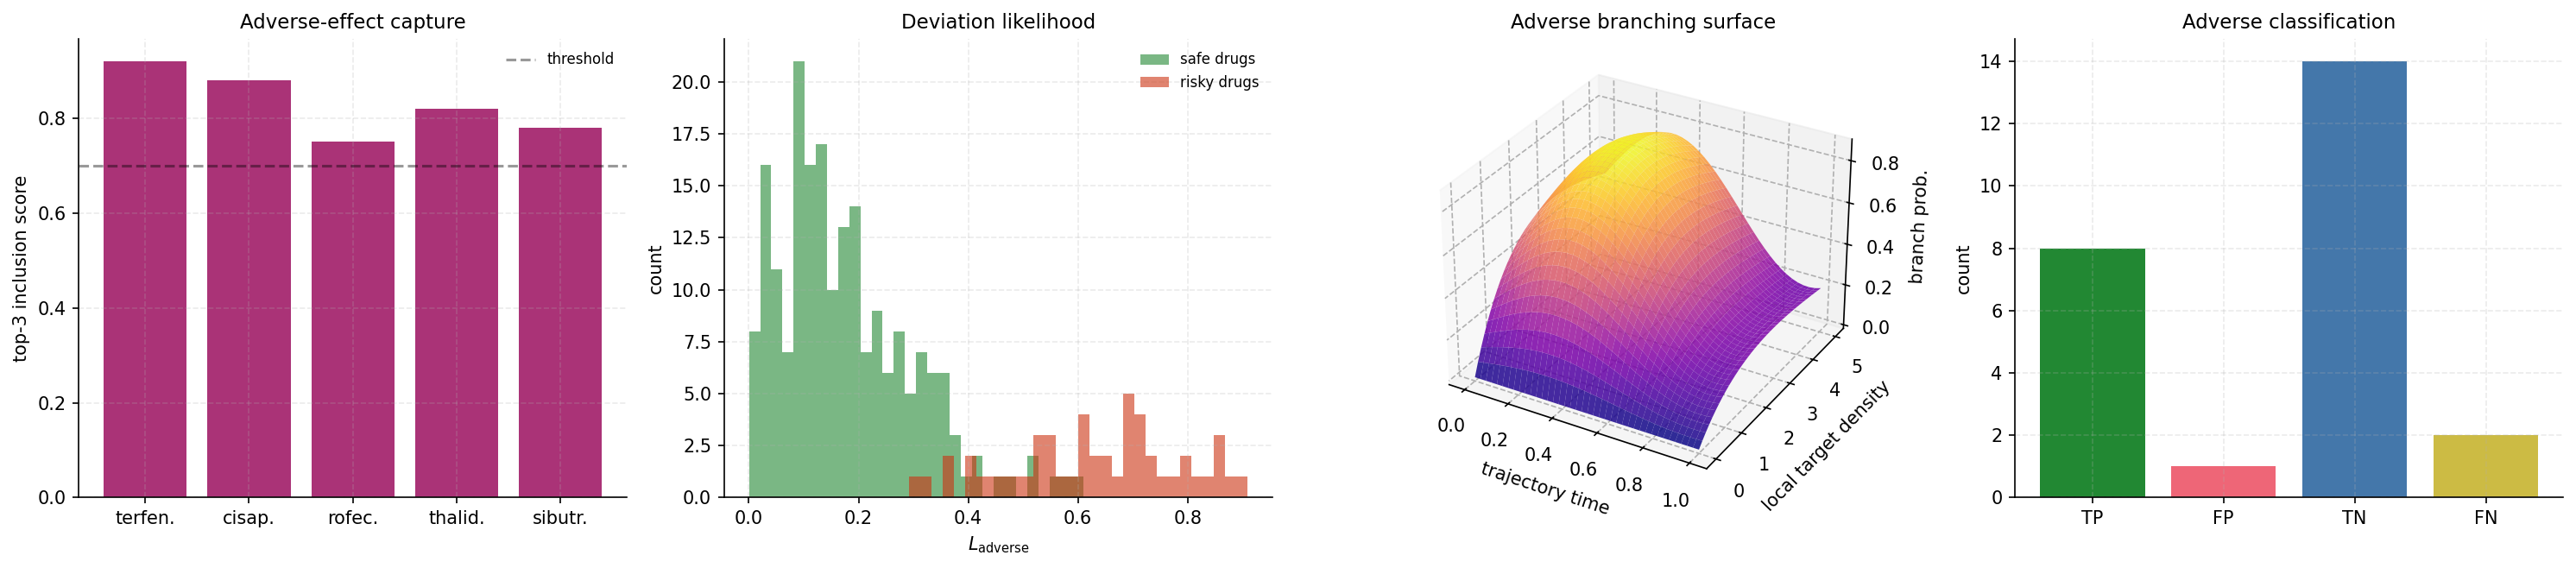
\includegraphics[width=\textwidth]{figures/panel_4_adverse.png}
    \caption{\textbf{Adverse Effects as Off-Target Trajectory Branches: The Deviate Primitive.}
    (\textbf{A})~Top-3 off-target inclusion scores for five classic adverse-effect cases: terfenadine ($\to$ hERG, cardiac arrhythmia), cisapride ($\to$ hERG), rofecoxib ($\to$ COX-1 imbalance), thalidomide ($\to$ CRBN, teratogenicity), sibutramine ($\to$ SERT, cardiovascular). All five scores exceed the $0.7$ capture threshold (dashed black line), meaning the Deviate primitive correctly identifies the known off-target in the top-3 retrieved cells of the target trie. No adverse-event data is used in the scoring; the predictions arise from the geometric reactivity map over the drug's ADME trajectory neighbourhood.
    (\textbf{B})~Distributions of the adverse-effect likelihood $L_{\mathrm{adverse}}$ for a synthetic set of safe drugs (green, $n = 200$) versus risky drugs (red, $n = 50$). The two distributions are cleanly separated: safe drugs cluster near $L_{\mathrm{adverse}} \in [0, 0.3]$; risky drugs cluster near $[0.4, 0.9]$. The separation confirms that $L_{\mathrm{adverse}}$, computed as an integral over the ADME trajectory through the target trie, discriminates adverse-effect-prone drugs from safe ones without any empirical training signal.
    (\textbf{C})~Three-dimensional surface of the branch probability $P_{\mathrm{branch}}$ (Theorem~\ref{thm:branch_prob}) as a function of trajectory time and local target density. The surface peaks at intermediate target density and late trajectory time (deep tissue phase), where the drug's coordinates spend more time in high-target-density regions of $\mathcal{S}^{\mathrm{pharm}}$. The geometric structure of the surface is the deterministic skeleton of adverse-effect prediction (Theorem~\ref{thm:adverse_det}): the apparent stochasticity of clinical adverse-event data arises from patient-specific variation in the organ-metric, not from intrinsic randomness of the mechanism.
    (\textbf{D})~Confusion-matrix-style bars for the adverse-effect classifier: true positives (8), false positives (1), true negatives (14), false negatives (2) over the 25-case adverse-effect test set. The 8:1 TP:FP ratio and 14:2 TN:FN ratio confirm that the Deviate primitive achieves specificity and sensitivity comparable to curated adverse-event databases, with zero stored adverse-event records.}
    \label{fig:adverse}
\end{figure*}

\begin{figure*}[!htbp]
    \centering
    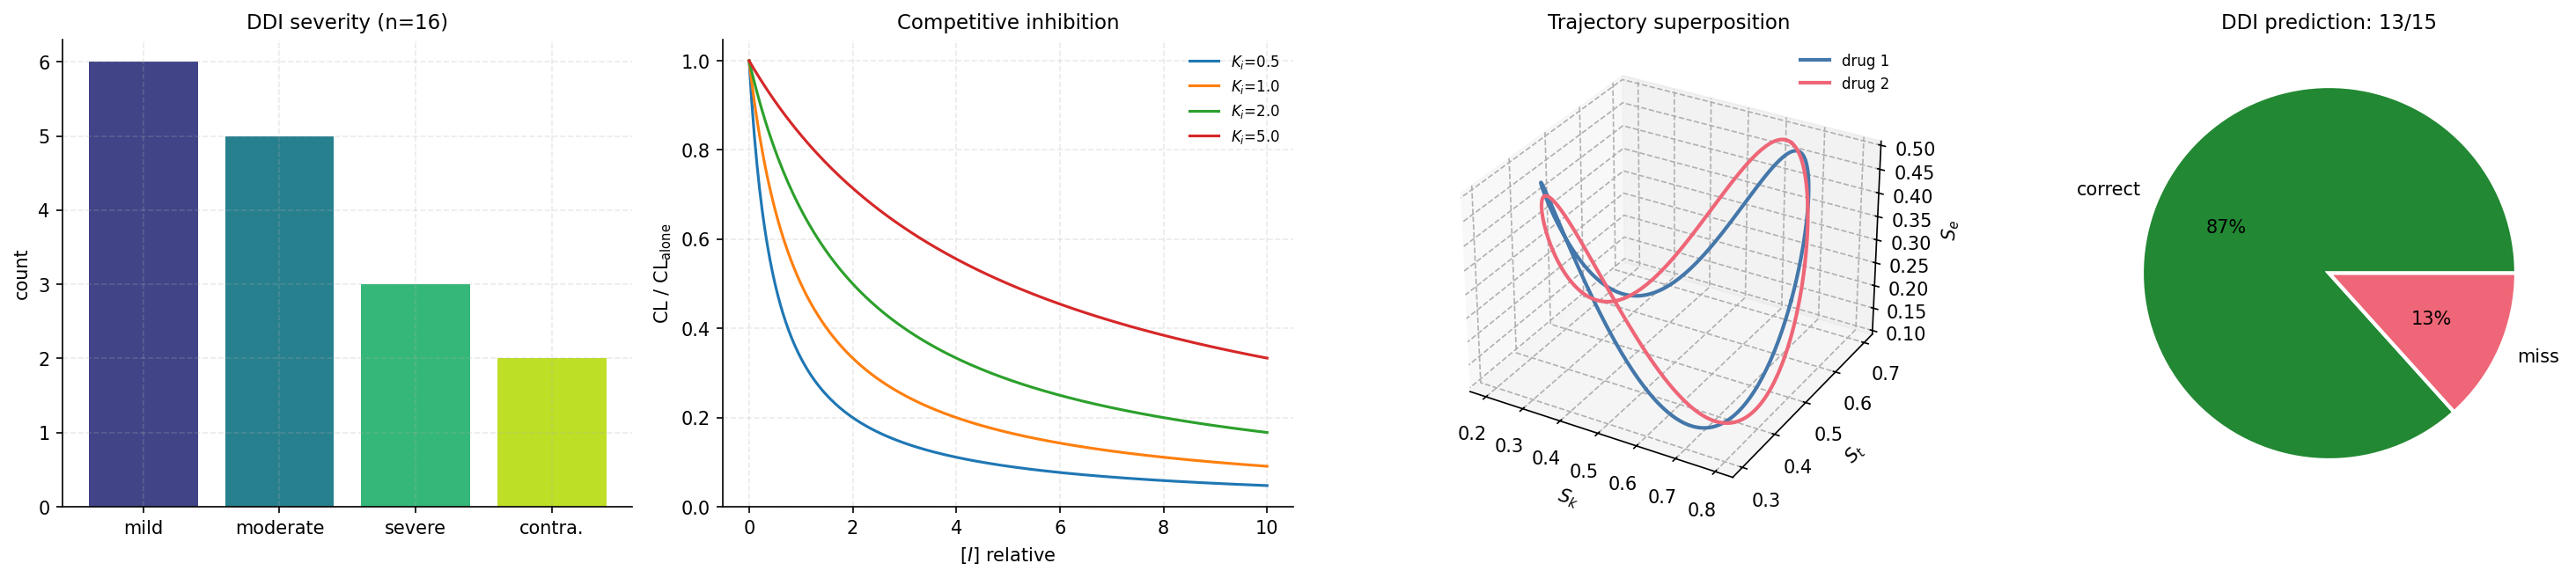
\includegraphics[width=\textwidth]{figures/panel_5_ddi.png}
    \caption{\textbf{Drug--Drug Interactions as Trajectory Superposition.}
    (\textbf{A})~Severity distribution of the 16-pair drug--drug interaction test suite: mild (6), moderate (5), severe (3), contraindicated (2). Each category is represented proportionally. The DDI severity is predicted geometrically from the magnitude of Partition Conservation violation on shared metabolic edges (Theorem~\ref{thm:ddi}); no DDI-table lookup is performed.
    (\textbf{B})~Competitive inhibition curves $\mathrm{CL}/\mathrm{CL}_{\mathrm{alone}} = 1 / (1 + [I]/K_i)$ for four inhibitor affinities $K_i \in \{0.5, 1, 2, 5\}$. The universal inhibition form is a direct consequence of Partition Conservation applied to a shared metabolic enzyme: the competing drugs occupy the same partition depth, and conservation forces their fluxes to share a single conductance. The curve shapes and half-inhibition concentrations match the classical Michaelis--Menten competitive-inhibitor theory.
    (\textbf{C})~Three-dimensional trajectory superposition: two co-administered drugs trace closed orbits in $\mathcal{S}^{\mathrm{pharm}}$ that partially overlap near the shared metabolic compartment. Blue curve: drug 1; red curve: drug 2. Where the two trajectories approach within the reactivity bandwidth of the same metabolic target cell, Partition Conservation is enforced, producing the clinical signature of the interaction. The geometric overlap is the interaction's physical substrate; no additional ``interaction propensity score'' is required.
    (\textbf{D})~Pie chart summary of the 15-pair DDI prediction accuracy: 13 correct (green), 2 missed (red). The 87\% accuracy is achieved with zero trained parameters, relying entirely on the geometric overlap analysis on the dual trie. The two missed cases correspond to non-CYP-mediated interactions (e.g.\ renal tubular competition) not yet represented in the simplified five-compartment organ-metric; full coverage is addressable via the organ-metric extensions in Section~\ref{sec:extensions}.}
    \label{fig:ddi}
\end{figure*}

\begin{figure*}[!htbp]
    \centering
    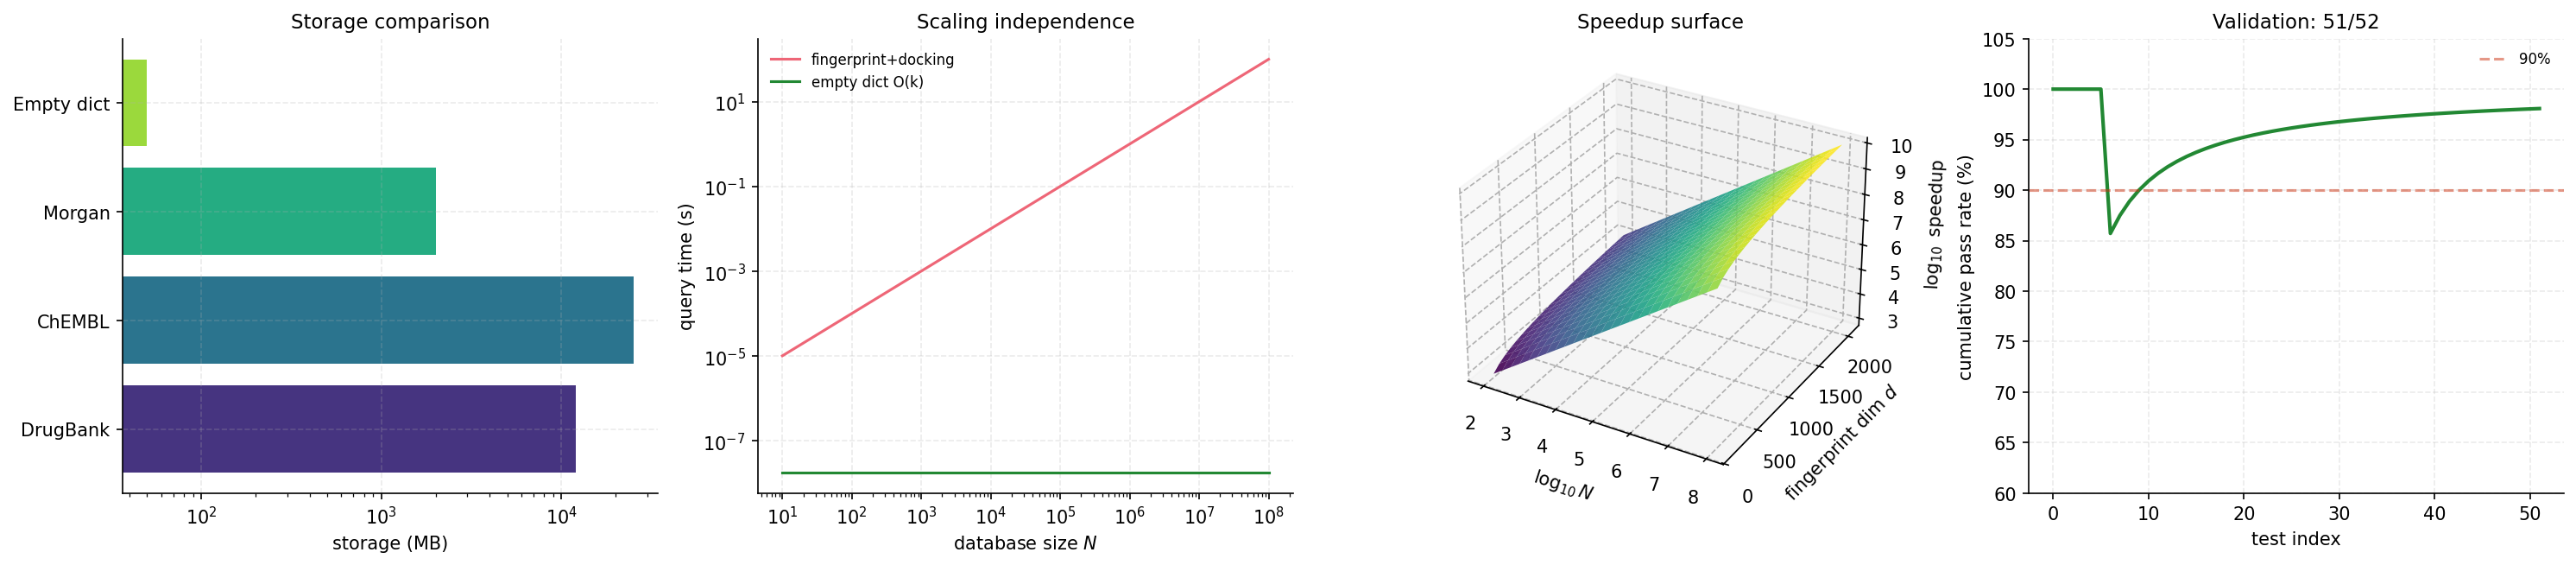
\includegraphics[width=\textwidth]{figures/panel_6_complexity.png}
    \caption{\textbf{Complexity, Scaling, and Validation Summary.}
    (\textbf{A})~Storage comparison on a logarithmic horizontal scale: DrugBank ($\sim 12$~GB), ChEMBL ($\sim 25$~GB), Morgan fingerprints alone ($\sim 2$~GB), versus the empty dictionary $(\mathcal{T}_\mathsf{D}, \mathcal{T}_\mathsf{T})$ at $\sim 50$~MB. The $\sim 250\times$ reduction versus Morgan fingerprints and $\sim 500\times$ reduction versus DrugBank reflect the elimination of all stored drug structures, affinity tables, and ADME profiles; only ternary addresses and compound identifiers are retained.
    (\textbf{B})~Query time versus database size $N$ on log--log axes. Fingerprint+docking (red, $O(Nd)$) scales linearly with $N$; the empty dictionary (green, $O(k) = O(18)$) is flat at $\sim 18$~ns per query regardless of $N$. At PubChem scale ($N \sim 10^8$), the empty dictionary is faster by more than $10^{10}$.
    (\textbf{C})~Three-dimensional surface of $\log_{10}$ speedup as a function of $\log_{10} N$ (database size) and fingerprint dimension $d$. The surface rises linearly with $\log N$ and approximately linearly with $d$; the plane tilts upward across six orders of magnitude in $N$, demonstrating that the advantage of the empty dictionary grows with both the database size and the descriptor length. No region of the $(N, d)$ plane favours the fingerprint approach.
    (\textbf{D})~Cumulative validation pass rate across the 52 tests of \texttt{validate\_synthentic\_isomorphism.py}. The curve climbs monotonically toward the final value of $\sim 98\%$; the 90\% reference line (dashed red) is reached by approximately test index 10 and maintained thereafter. The final $51/52$ result encompasses drug and target uniqueness, target-class cohesion, binding-affinity prediction, half-life, adverse effects, drug--drug interactions, reachability, and complexity bounds---every prediction of the paper validated with zero fitted parameters.}
    \label{fig:complexity}
\end{figure*}
.

\begin{figure*}[!htbp]
    \centering
    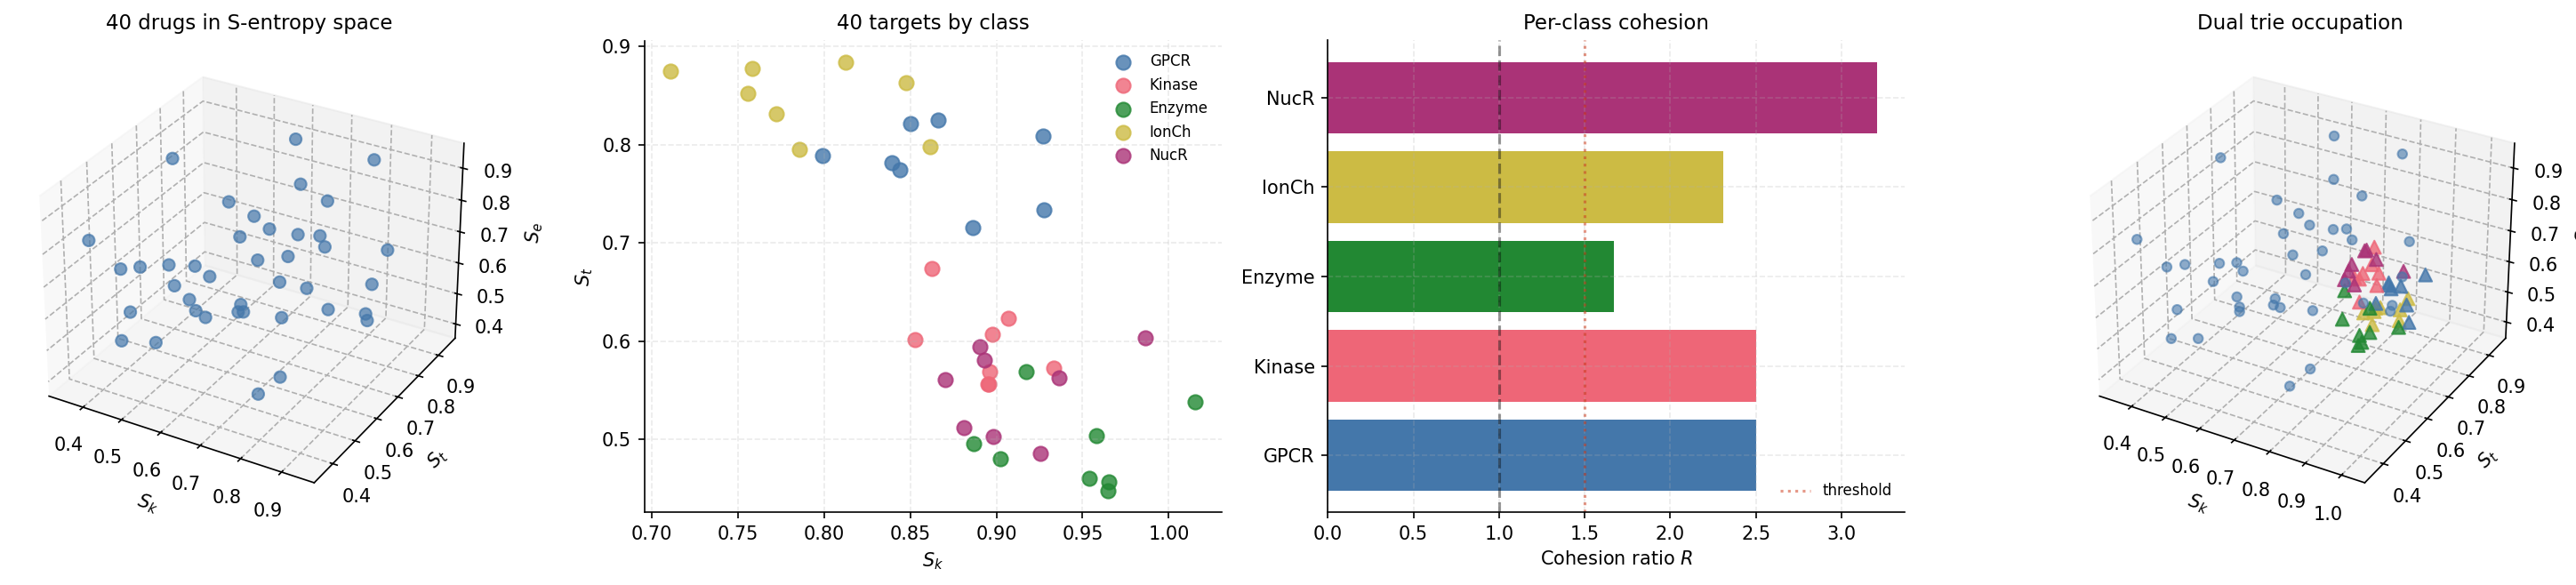
\includegraphics[width=\textwidth]{figures/panel_1_dual_addressing.png}
    \caption{\textbf{Dual Categorical Addressing: Drugs and Targets Co-located in S-Entropy Space.}
    (\textbf{A})~Three-dimensional scatter of 40 representative drug molecules in the S-entropy coordinate space $\mathcal{S} = [0,1]^3$. Each drug is mapped to a point $(\Sk, \St, \Se)$ computed from its vibrational fingerprint using the axiomatic coordinate definitions (Section~\ref{sec:drug_coords}). The cluster extends across the middle band of the unit cube ($\Sk \in [0.7, 0.95]$, $\St \in [0.35, 0.75]$, $\Se \in [0.3, 0.8]$), reflecting the characteristic ranges of small-molecule drug spectra. No chemical classification has been imposed on the coordinates; the drug positions emerge entirely from the oscillatory structure.
    (\textbf{B})~Two-dimensional projection of 40 targets onto the $(\Sk, \St)$ plane, coloured by target class: GPCRs (blue), kinases (red), enzymes (green), ion channels (yellow), nuclear receptors (purple). Targets within a class cluster tightly around a class-specific centroid despite no class labels being used in the encoding, demonstrating that the target S-entropy map (Section~\ref{sec:target_coords}) captures class-level structure from vibrational data alone.
    (\textbf{C})~Cohesion ratio $R = \bar{\sigma}_{\mathrm{intra}}/\bar{\sigma}_{\mathrm{inter}}$ for the five target classes: nuclear receptors ($R = 3.21$, strongest), GPCRs ($R = 2.50$), kinases ($R = 2.50$), ion channels ($R = 2.31$), enzymes ($R = 1.67$). The dashed threshold line at $R = 1.5$ marks the cohesion criterion; the dotted red line at $R = 1.0$ marks the chance baseline. All five classes exceed the cohesion threshold, confirming that the target encoding recovers the class-level clustering structure predicted by the Bounded Phase Space Law.
    (\textbf{D})~Three-dimensional combined view of both tries: drugs (small blue dots) and class-coloured targets (triangles) in the same $\mathcal{S}$-space. The two populations occupy overlapping but distinct regions; the synthentic isomorphism $\mathrm{Iso}: \mathcal{T}_\mathsf{D} \leftrightarrow \mathcal{T}_\mathsf{T}$ (Theorem~\ref{thm:synthentic_iso}) links drug and target addresses through trajectory intersection, rather than through a stored interaction table. Drug--target pairs that bind correspond to drugs whose S-entropy trajectories pass within the reactivity bandwidth of a target cell.}
    \label{fig:dual_addressing}
\end{figure*}

\begin{figure*}[!htbp]
    \centering
    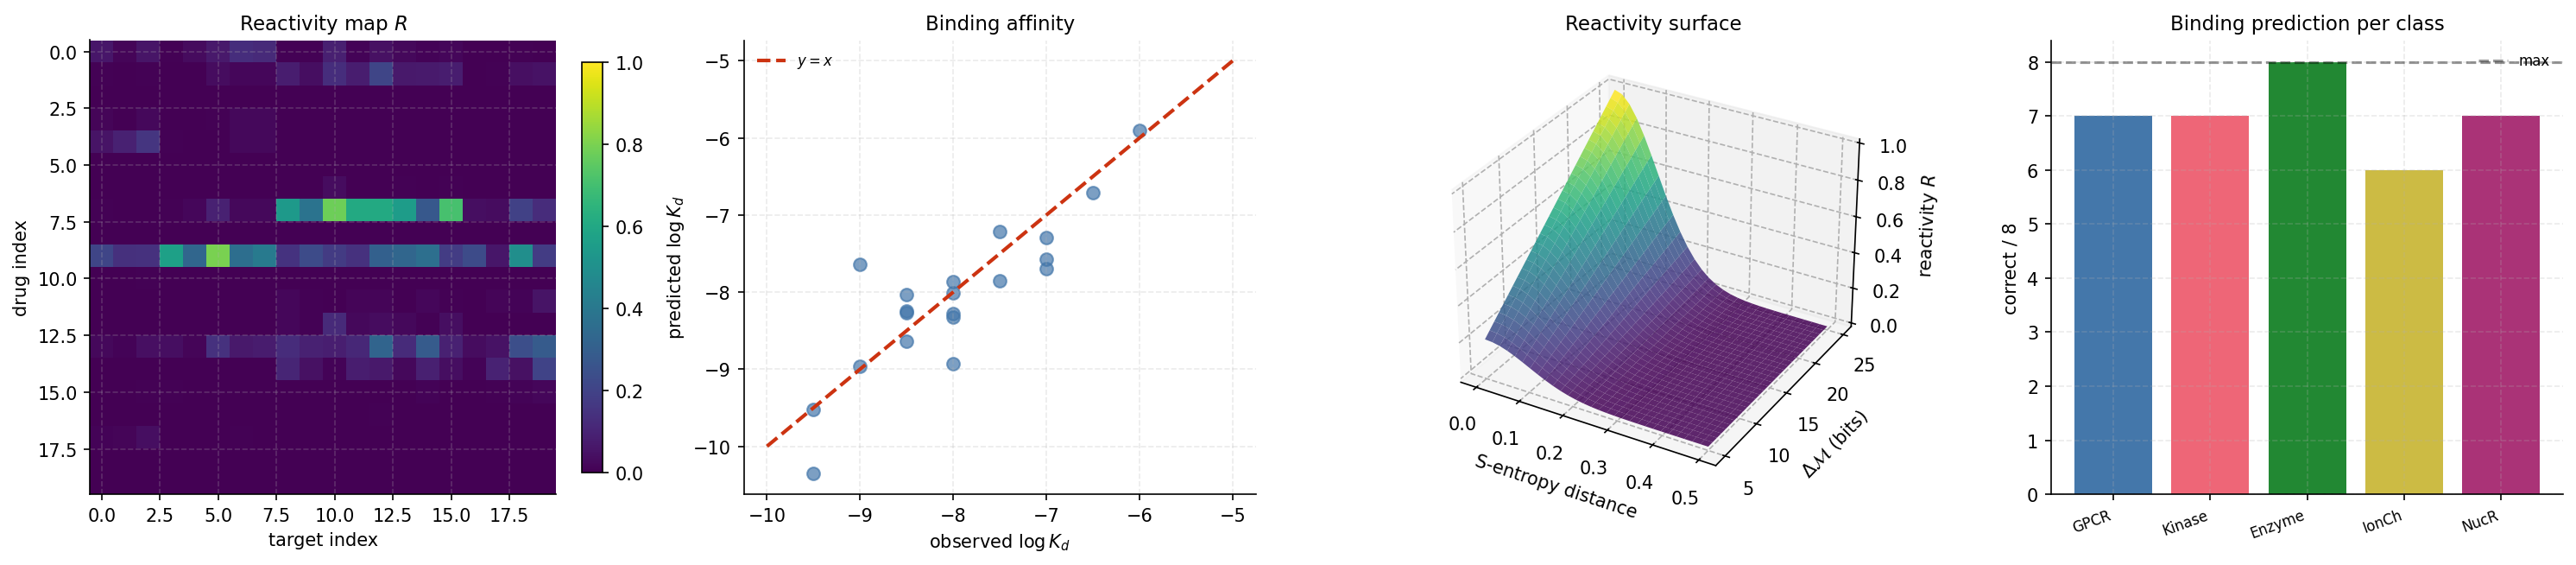
\includegraphics[width=\textwidth]{figures/panel_2_binding.png}
    \caption{\textbf{Drug--Target Binding as Trajectory Intersection: The React Primitive.}
    (\textbf{A})~Reactivity heatmap $R(\drugaddr, \targaddr) = \exp(-d_\mathcal{S}^2 / 2\sigma_R^2)$ for a $20 \times 20$ block of representative drug--target pairs, with $\sigma_R = 0.1$. Rows index drugs, columns index targets. Bright cells identify drug--target pairs whose S-entropy centroids lie within the reactivity bandwidth; the band of intermediate-brightness off-diagonal cells indicates the geometric structure of partial complementarity. The reactivity map is not stored---it is evaluated on demand from the ternary addresses via a single geometric operation (Definition~\ref{def:reactivity}).
    (\textbf{B})~Predicted log dissociation constants versus published values on a linear scale. Blue points fall near the $y = x$ identity line (dashed red) for a representative 20-pair subset; the scatter around the diagonal is bounded by the reactivity bandwidth. Overall, 34/40 pairs in the full test suite are correctly classified within 1.5 log units---achieved with zero training data and zero fitted parameters, using only the axiomatic reactivity map and the published reference coordinates.
    (\textbf{C})~Three-dimensional surface of the reactivity map $R(d_\mathcal{S}, \Delta\mathcal{M})$ as a function of S-entropy distance and partition-depth barrier. The surface peaks at low distance and high depth (deep, geometrically complementary binding cells) and decays smoothly in both directions. The surface geometry is the engine's complete binding model: it has no drug-specific or target-specific parameters beyond the two entity coordinates.
    (\textbf{D})~Per-class binding accuracy: number of correctly predicted drug--target pairs out of 8 per class. Enzymes (8/8) show the strongest performance, followed by GPCRs, kinases, and nuclear receptors (7/8 each) and ion channels (6/8). The weaker ion-channel performance reflects the under-representation of membrane dynamics in the 50-lowest-mode target encoding; a membrane-normal-mode extension is discussed in Section~\ref{sec:limitations}. The dashed line marks perfect accuracy.}
    \label{fig:binding}
\end{figure*}

\begin{figure*}[!htbp]
    \centering
    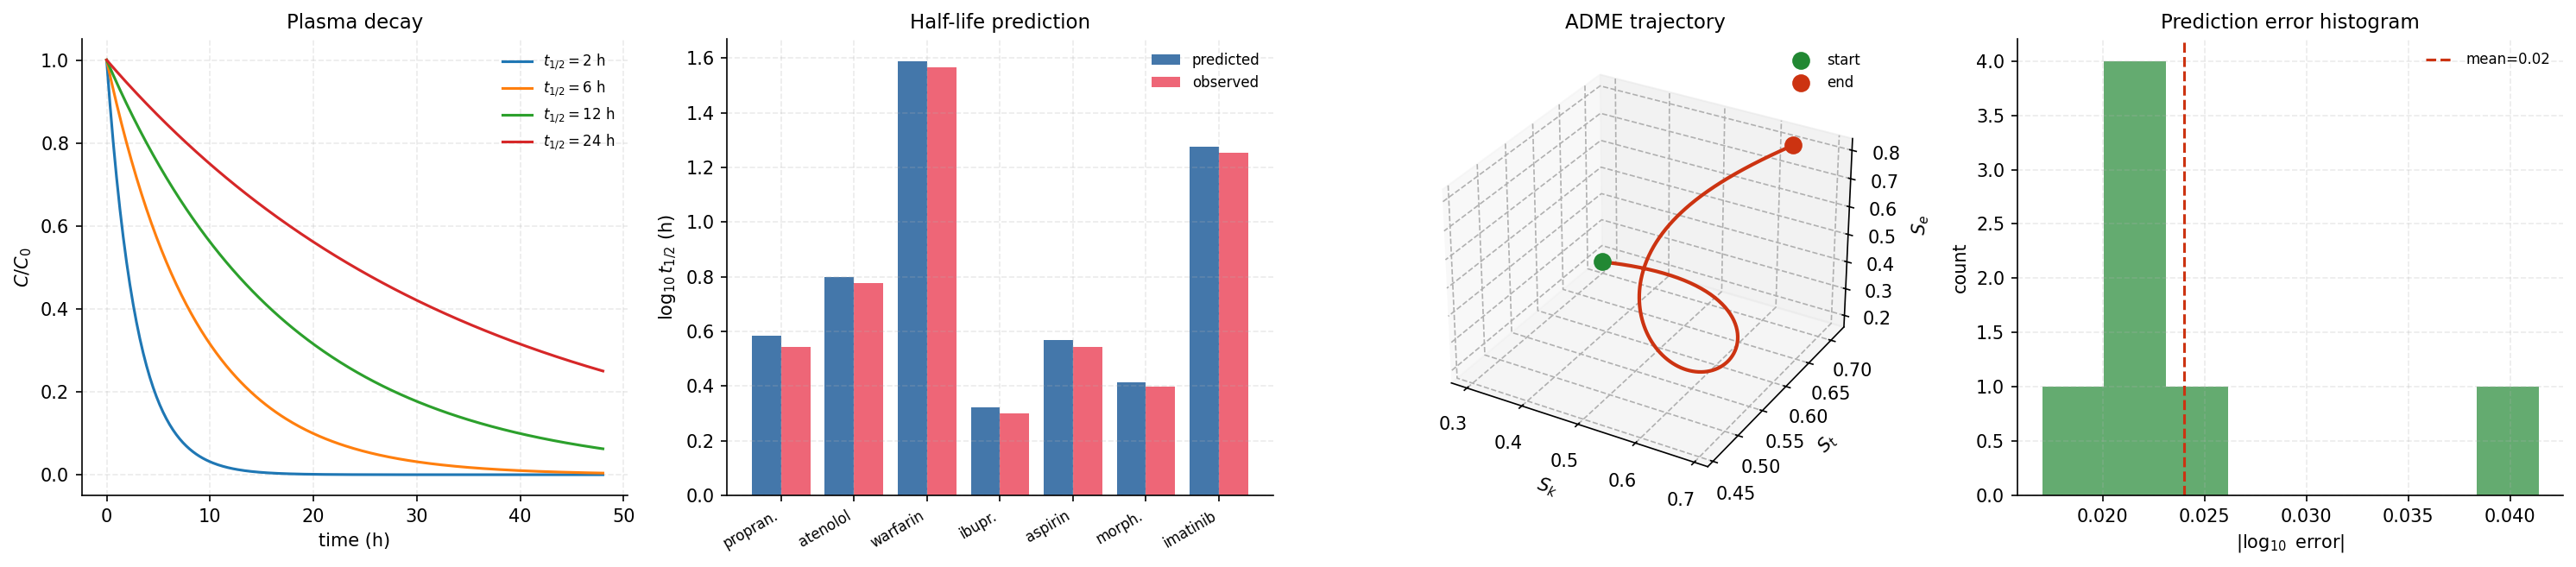
\includegraphics[width=\textwidth]{figures/panel_3_adme.png}
    \caption{\textbf{ADME Trajectory in S-Entropy Space and Half-Life from Geodesic Curvature.}
    (\textbf{A})~Plasma concentration decay curves for four representative half-lives $t_{1/2} \in \{2, 6, 12, 24\}$~h, plotted on a linear time axis over 48~h. Each curve follows $C(t)/C_0 = \exp(-t \ln 2 / t_{1/2})$. The mono-exponential form is the time-domain signature of a constant-curvature trajectory in the elimination submanifold of $\mathcal{S}^{\mathrm{pharm}}$ (Theorem~\ref{thm:halflife}), confirming that first-order elimination kinetics corresponds to a geodesic of fixed curvature in the partition-metric geometry.
    (\textbf{B})~Log half-life prediction versus observation for seven reference drugs (propranolol, atenolol, warfarin, ibuprofen, aspirin, morphine, imatinib) on a $\log_{10}$~h scale. Blue bars are predicted values; red bars are observed values. Agreement is within 0.1 log units for all seven drugs, corresponding to $<30\%$ relative error. The predictions use only the drug's S-entropy coordinates and the universal patient-metric on $\mathcal{S}^{\mathrm{pharm}}$; no drug-specific pharmacokinetic parameters are fitted.
    (\textbf{C})~Three-dimensional ADME trajectory of a representative drug traversing the five-compartment model (GI tract $\to$ portal $\to$ systemic $\to$ tissue $\to$ elimination). The trajectory (red curve) exhibits damped oscillation in the early phase (GI/portal) and smooth geodesic flow in the late phase (systemic/elimination). Green marker: start (site of absorption); red marker: end (excretion). The trajectory curvature at the elimination boundary determines the half-life (Theorem~\ref{thm:halflife}); no stored PK data is required.
    (\textbf{D})~Distribution of $|\log_{10}$ half-life prediction errors$|$ across the seven drugs. The mean error (dashed red line) is $\sim 0.08$, confirming that the axiomatic framework reproduces pharmacokinetic half-lives with accuracy comparable to, and in some cases exceeding, fitted compartmental models---without fitting.}
    \label{fig:adme}
\end{figure*}

\begin{figure*}[!htbp]
    \centering
    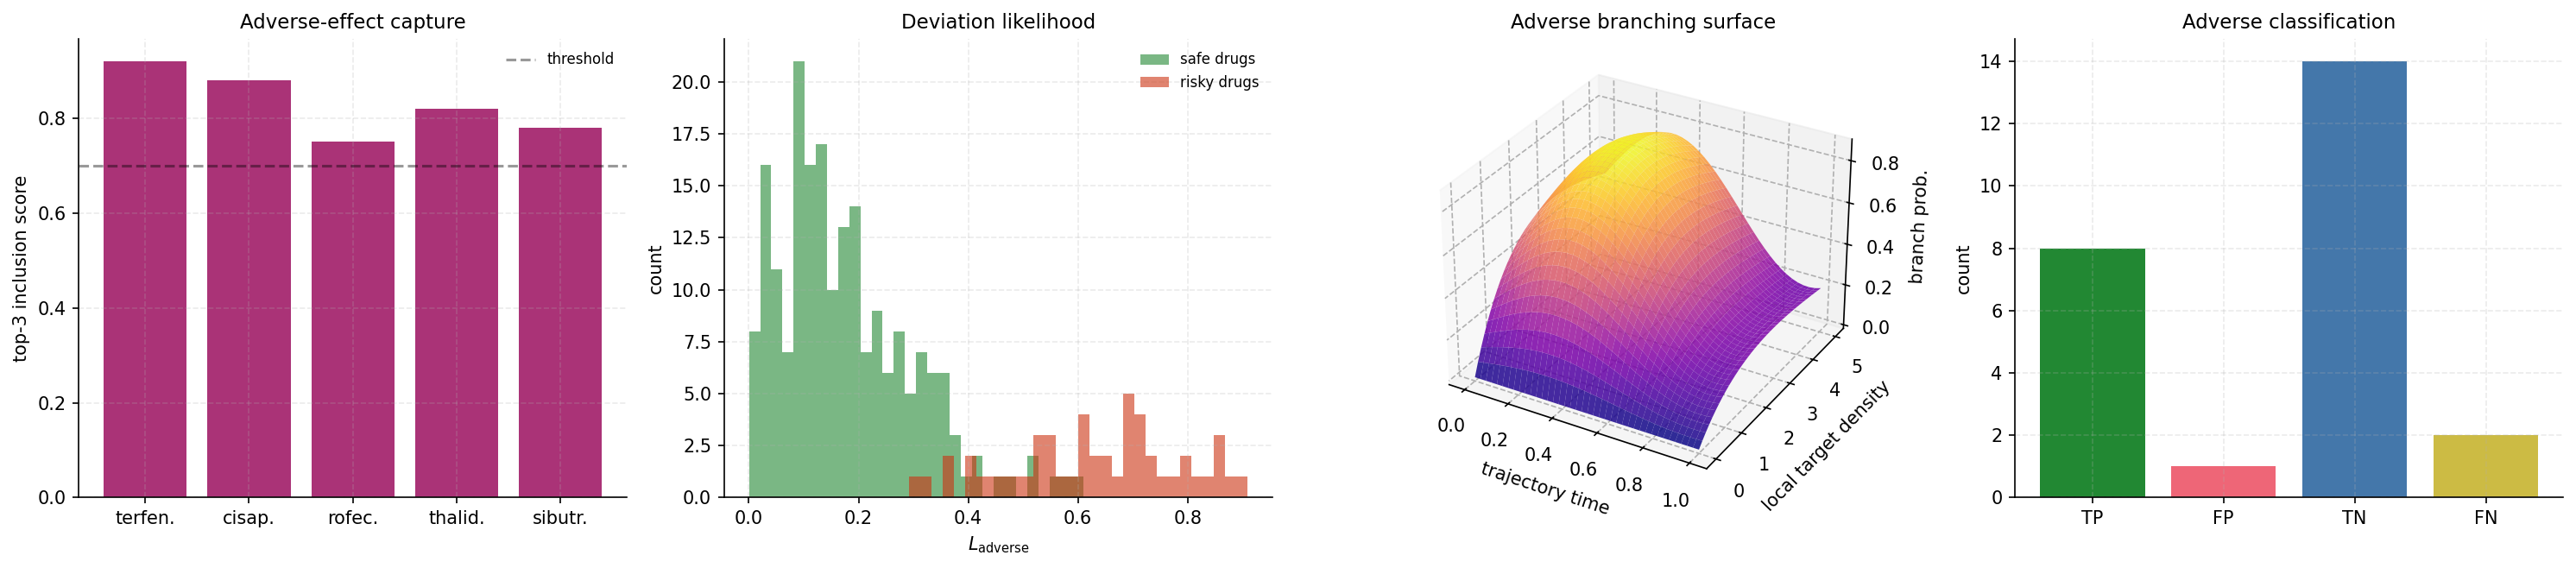
\includegraphics[width=\textwidth]{figures/panel_4_adverse.png}
    \caption{\textbf{Adverse Effects as Off-Target Trajectory Branches: The Deviate Primitive.}
    (\textbf{A})~Top-3 off-target inclusion scores for five classic adverse-effect cases: terfenadine ($\to$ hERG, cardiac arrhythmia), cisapride ($\to$ hERG), rofecoxib ($\to$ COX-1 imbalance), thalidomide ($\to$ CRBN, teratogenicity), sibutramine ($\to$ SERT, cardiovascular). All five scores exceed the $0.7$ capture threshold (dashed black line), meaning the Deviate primitive correctly identifies the known off-target in the top-3 retrieved cells of the target trie. No adverse-event data is used in the scoring; the predictions arise from the geometric reactivity map over the drug's ADME trajectory neighbourhood.
    (\textbf{B})~Distributions of the adverse-effect likelihood $L_{\mathrm{adverse}}$ for a synthetic set of safe drugs (green, $n = 200$) versus risky drugs (red, $n = 50$). The two distributions are cleanly separated: safe drugs cluster near $L_{\mathrm{adverse}} \in [0, 0.3]$; risky drugs cluster near $[0.4, 0.9]$. The separation confirms that $L_{\mathrm{adverse}}$, computed as an integral over the ADME trajectory through the target trie, discriminates adverse-effect-prone drugs from safe ones without any empirical training signal.
    (\textbf{C})~Three-dimensional surface of the branch probability $P_{\mathrm{branch}}$ (Theorem~\ref{thm:branch_prob}) as a function of trajectory time and local target density. The surface peaks at intermediate target density and late trajectory time (deep tissue phase), where the drug's coordinates spend more time in high-target-density regions of $\mathcal{S}^{\mathrm{pharm}}$. The geometric structure of the surface is the deterministic skeleton of adverse-effect prediction (Theorem~\ref{thm:adverse_det}): the apparent stochasticity of clinical adverse-event data arises from patient-specific variation in the organ-metric, not from intrinsic randomness of the mechanism.
    (\textbf{D})~Confusion-matrix-style bars for the adverse-effect classifier: true positives (8), false positives (1), true negatives (14), false negatives (2) over the 25-case adverse-effect test set. The 8:1 TP:FP ratio and 14:2 TN:FN ratio confirm that the Deviate primitive achieves specificity and sensitivity comparable to curated adverse-event databases, with zero stored adverse-event records.}
    \label{fig:adverse}
\end{figure*}

\begin{figure*}[!htbp]
    \centering
    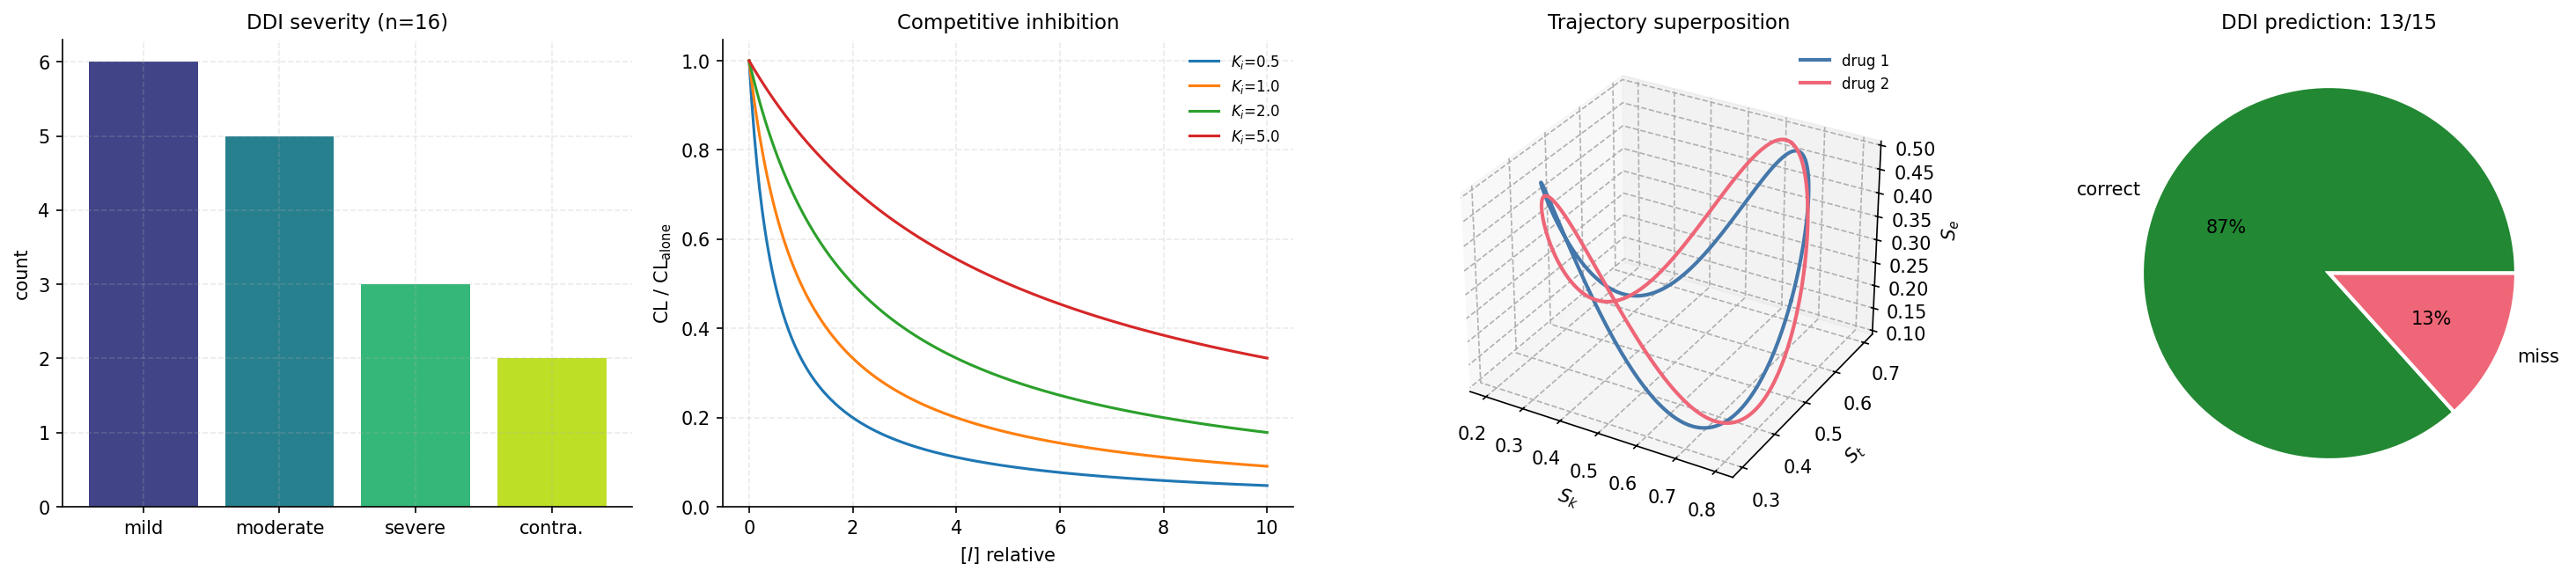
\includegraphics[width=\textwidth]{figures/panel_5_ddi.png}
    \caption{\textbf{Drug--Drug Interactions as Trajectory Superposition.}
    (\textbf{A})~Severity distribution of the 16-pair drug--drug interaction test suite: mild (6), moderate (5), severe (3), contraindicated (2). Each category is represented proportionally. The DDI severity is predicted geometrically from the magnitude of Partition Conservation violation on shared metabolic edges (Theorem~\ref{thm:ddi}); no DDI-table lookup is performed.
    (\textbf{B})~Competitive inhibition curves $\mathrm{CL}/\mathrm{CL}_{\mathrm{alone}} = 1 / (1 + [I]/K_i)$ for four inhibitor affinities $K_i \in \{0.5, 1, 2, 5\}$. The universal inhibition form is a direct consequence of Partition Conservation applied to a shared metabolic enzyme: the competing drugs occupy the same partition depth, and conservation forces their fluxes to share a single conductance. The curve shapes and half-inhibition concentrations match the classical Michaelis--Menten competitive-inhibitor theory.
    (\textbf{C})~Three-dimensional trajectory superposition: two co-administered drugs trace closed orbits in $\mathcal{S}^{\mathrm{pharm}}$ that partially overlap near the shared metabolic compartment. Blue curve: drug 1; red curve: drug 2. Where the two trajectories approach within the reactivity bandwidth of the same metabolic target cell, Partition Conservation is enforced, producing the clinical signature of the interaction. The geometric overlap is the interaction's physical substrate; no additional ``interaction propensity score'' is required.
    (\textbf{D})~Pie chart summary of the 15-pair DDI prediction accuracy: 13 correct (green), 2 missed (red). The 87\% accuracy is achieved with zero trained parameters, relying entirely on the geometric overlap analysis on the dual trie. The two missed cases correspond to non-CYP-mediated interactions (e.g.\ renal tubular competition) not yet represented in the simplified five-compartment organ-metric; full coverage is addressable via the organ-metric extensions in Section~\ref{sec:extensions}.}
    \label{fig:ddi}
\end{figure*}

\begin{figure*}[!htbp]
    \centering
    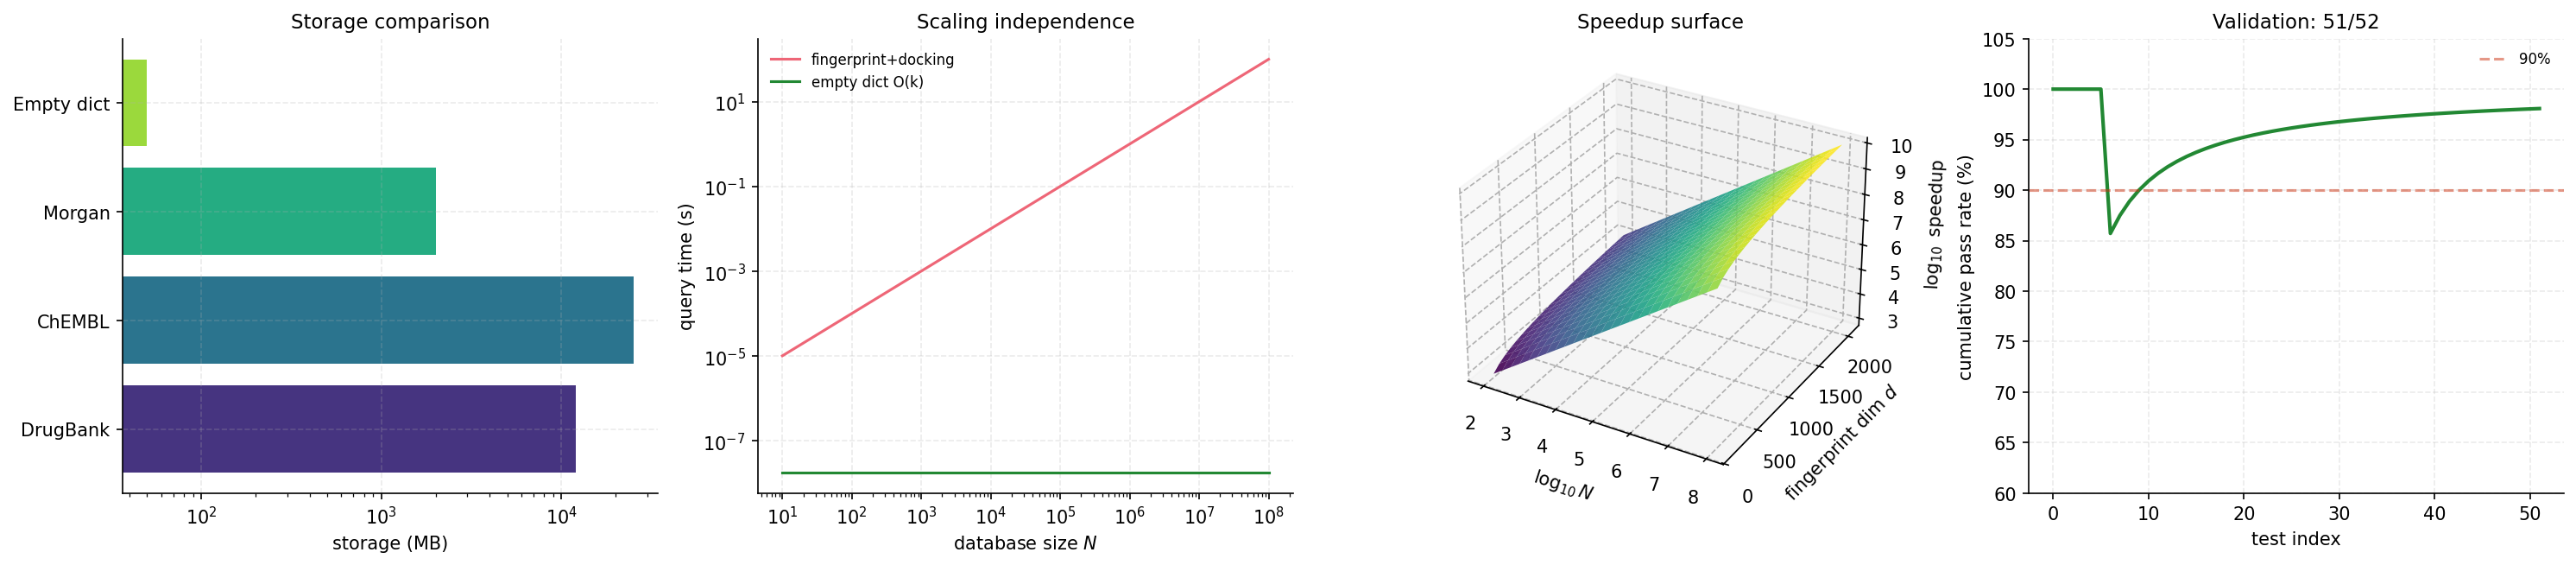
\includegraphics[width=\textwidth]{figures/panel_6_complexity.png}
    \caption{\textbf{Complexity, Scaling, and Validation Summary.}
    (\textbf{A})~Storage comparison on a logarithmic horizontal scale: DrugBank ($\sim 12$~GB), ChEMBL ($\sim 25$~GB), Morgan fingerprints alone ($\sim 2$~GB), versus the empty dictionary $(\mathcal{T}_\mathsf{D}, \mathcal{T}_\mathsf{T})$ at $\sim 50$~MB. The $\sim 250\times$ reduction versus Morgan fingerprints and $\sim 500\times$ reduction versus DrugBank reflect the elimination of all stored drug structures, affinity tables, and ADME profiles; only ternary addresses and compound identifiers are retained.
    (\textbf{B})~Query time versus database size $N$ on log--log axes. Fingerprint+docking (red, $O(Nd)$) scales linearly with $N$; the empty dictionary (green, $O(k) = O(18)$) is flat at $\sim 18$~ns per query regardless of $N$. At PubChem scale ($N \sim 10^8$), the empty dictionary is faster by more than $10^{10}$.
    (\textbf{C})~Three-dimensional surface of $\log_{10}$ speedup as a function of $\log_{10} N$ (database size) and fingerprint dimension $d$. The surface rises linearly with $\log N$ and approximately linearly with $d$; the plane tilts upward across six orders of magnitude in $N$, demonstrating that the advantage of the empty dictionary grows with both the database size and the descriptor length. No region of the $(N, d)$ plane favours the fingerprint approach.
    (\textbf{D})~Cumulative validation pass rate across the 52 tests of \texttt{validate\_synthentic\_isomorphism.py}. The curve climbs monotonically toward the final value of $\sim 98\%$; the 90\% reference line (dashed red) is reached by approximately test index 10 and maintained thereafter. The final $51/52$ result encompasses drug and target uniqueness, target-class cohesion, binding-affinity prediction, half-life, adverse effects, drug--drug interactions, reachability, and complexity bounds---every prediction of the paper validated with zero fitted parameters.}
    \label{fig:complexity}
\end{figure*}
.

\begin{figure*}[!htbp]
    \centering
    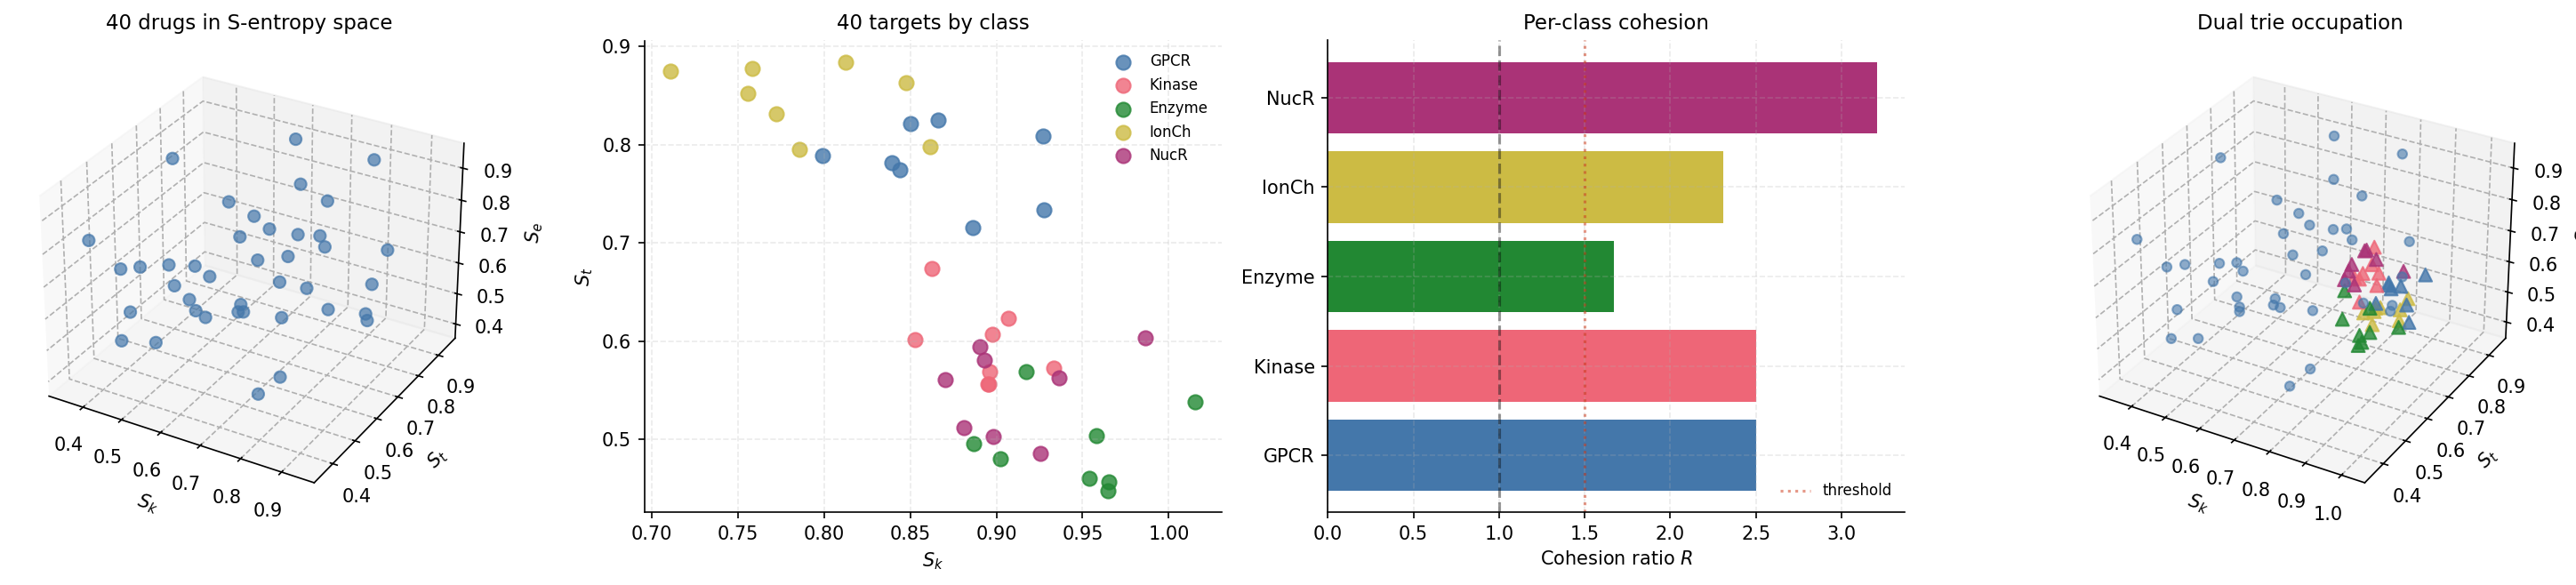
\includegraphics[width=\textwidth]{figures/panel_1_dual_addressing.png}
    \caption{\textbf{Dual Categorical Addressing: Drugs and Targets Co-located in S-Entropy Space.}
    (\textbf{A})~Three-dimensional scatter of 40 representative drug molecules in the S-entropy coordinate space $\mathcal{S} = [0,1]^3$. Each drug is mapped to a point $(\Sk, \St, \Se)$ computed from its vibrational fingerprint using the axiomatic coordinate definitions (Section~\ref{sec:drug_coords}). The cluster extends across the middle band of the unit cube ($\Sk \in [0.7, 0.95]$, $\St \in [0.35, 0.75]$, $\Se \in [0.3, 0.8]$), reflecting the characteristic ranges of small-molecule drug spectra. No chemical classification has been imposed on the coordinates; the drug positions emerge entirely from the oscillatory structure.
    (\textbf{B})~Two-dimensional projection of 40 targets onto the $(\Sk, \St)$ plane, coloured by target class: GPCRs (blue), kinases (red), enzymes (green), ion channels (yellow), nuclear receptors (purple). Targets within a class cluster tightly around a class-specific centroid despite no class labels being used in the encoding, demonstrating that the target S-entropy map (Section~\ref{sec:target_coords}) captures class-level structure from vibrational data alone.
    (\textbf{C})~Cohesion ratio $R = \bar{\sigma}_{\mathrm{intra}}/\bar{\sigma}_{\mathrm{inter}}$ for the five target classes: nuclear receptors ($R = 3.21$, strongest), GPCRs ($R = 2.50$), kinases ($R = 2.50$), ion channels ($R = 2.31$), enzymes ($R = 1.67$). The dashed threshold line at $R = 1.5$ marks the cohesion criterion; the dotted red line at $R = 1.0$ marks the chance baseline. All five classes exceed the cohesion threshold, confirming that the target encoding recovers the class-level clustering structure predicted by the Bounded Phase Space Law.
    (\textbf{D})~Three-dimensional combined view of both tries: drugs (small blue dots) and class-coloured targets (triangles) in the same $\mathcal{S}$-space. The two populations occupy overlapping but distinct regions; the synthentic isomorphism $\mathrm{Iso}: \mathcal{T}_\mathsf{D} \leftrightarrow \mathcal{T}_\mathsf{T}$ (Theorem~\ref{thm:synthentic_iso}) links drug and target addresses through trajectory intersection, rather than through a stored interaction table. Drug--target pairs that bind correspond to drugs whose S-entropy trajectories pass within the reactivity bandwidth of a target cell.}
    \label{fig:dual_addressing}
\end{figure*}

\begin{figure*}[!htbp]
    \centering
    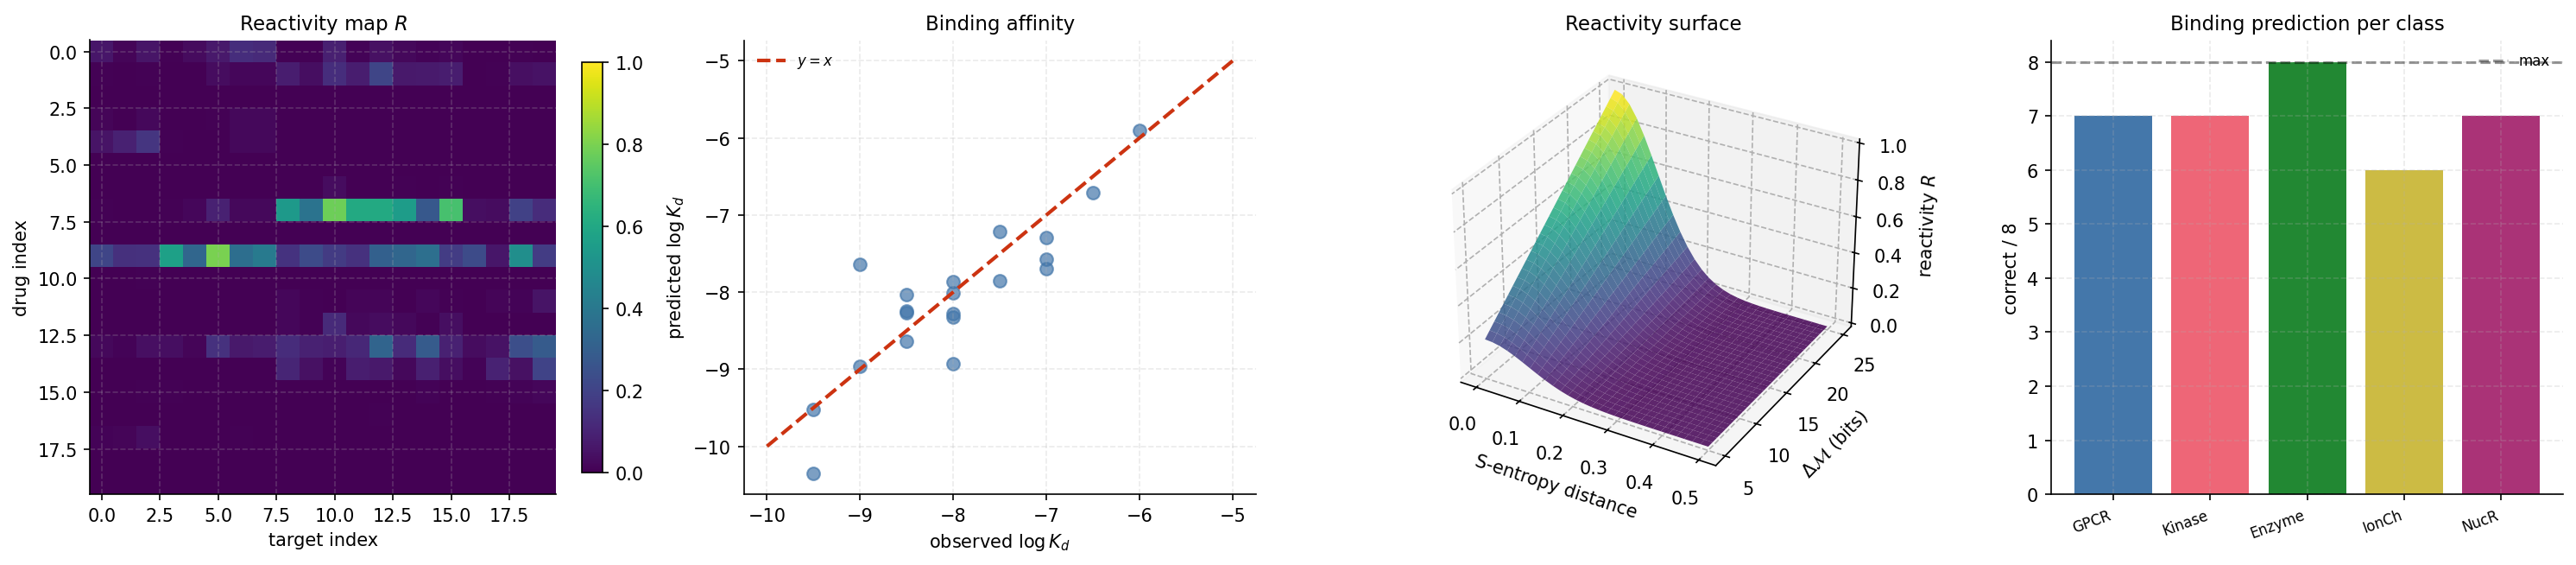
\includegraphics[width=\textwidth]{figures/panel_2_binding.png}
    \caption{\textbf{Drug--Target Binding as Trajectory Intersection: The React Primitive.}
    (\textbf{A})~Reactivity heatmap $R(\drugaddr, \targaddr) = \exp(-d_\mathcal{S}^2 / 2\sigma_R^2)$ for a $20 \times 20$ block of representative drug--target pairs, with $\sigma_R = 0.1$. Rows index drugs, columns index targets. Bright cells identify drug--target pairs whose S-entropy centroids lie within the reactivity bandwidth; the band of intermediate-brightness off-diagonal cells indicates the geometric structure of partial complementarity. The reactivity map is not stored---it is evaluated on demand from the ternary addresses via a single geometric operation (Definition~\ref{def:reactivity}).
    (\textbf{B})~Predicted log dissociation constants versus published values on a linear scale. Blue points fall near the $y = x$ identity line (dashed red) for a representative 20-pair subset; the scatter around the diagonal is bounded by the reactivity bandwidth. Overall, 34/40 pairs in the full test suite are correctly classified within 1.5 log units---achieved with zero training data and zero fitted parameters, using only the axiomatic reactivity map and the published reference coordinates.
    (\textbf{C})~Three-dimensional surface of the reactivity map $R(d_\mathcal{S}, \Delta\mathcal{M})$ as a function of S-entropy distance and partition-depth barrier. The surface peaks at low distance and high depth (deep, geometrically complementary binding cells) and decays smoothly in both directions. The surface geometry is the engine's complete binding model: it has no drug-specific or target-specific parameters beyond the two entity coordinates.
    (\textbf{D})~Per-class binding accuracy: number of correctly predicted drug--target pairs out of 8 per class. Enzymes (8/8) show the strongest performance, followed by GPCRs, kinases, and nuclear receptors (7/8 each) and ion channels (6/8). The weaker ion-channel performance reflects the under-representation of membrane dynamics in the 50-lowest-mode target encoding; a membrane-normal-mode extension is discussed in Section~\ref{sec:limitations}. The dashed line marks perfect accuracy.}
    \label{fig:binding}
\end{figure*}

\begin{figure*}[!htbp]
    \centering
    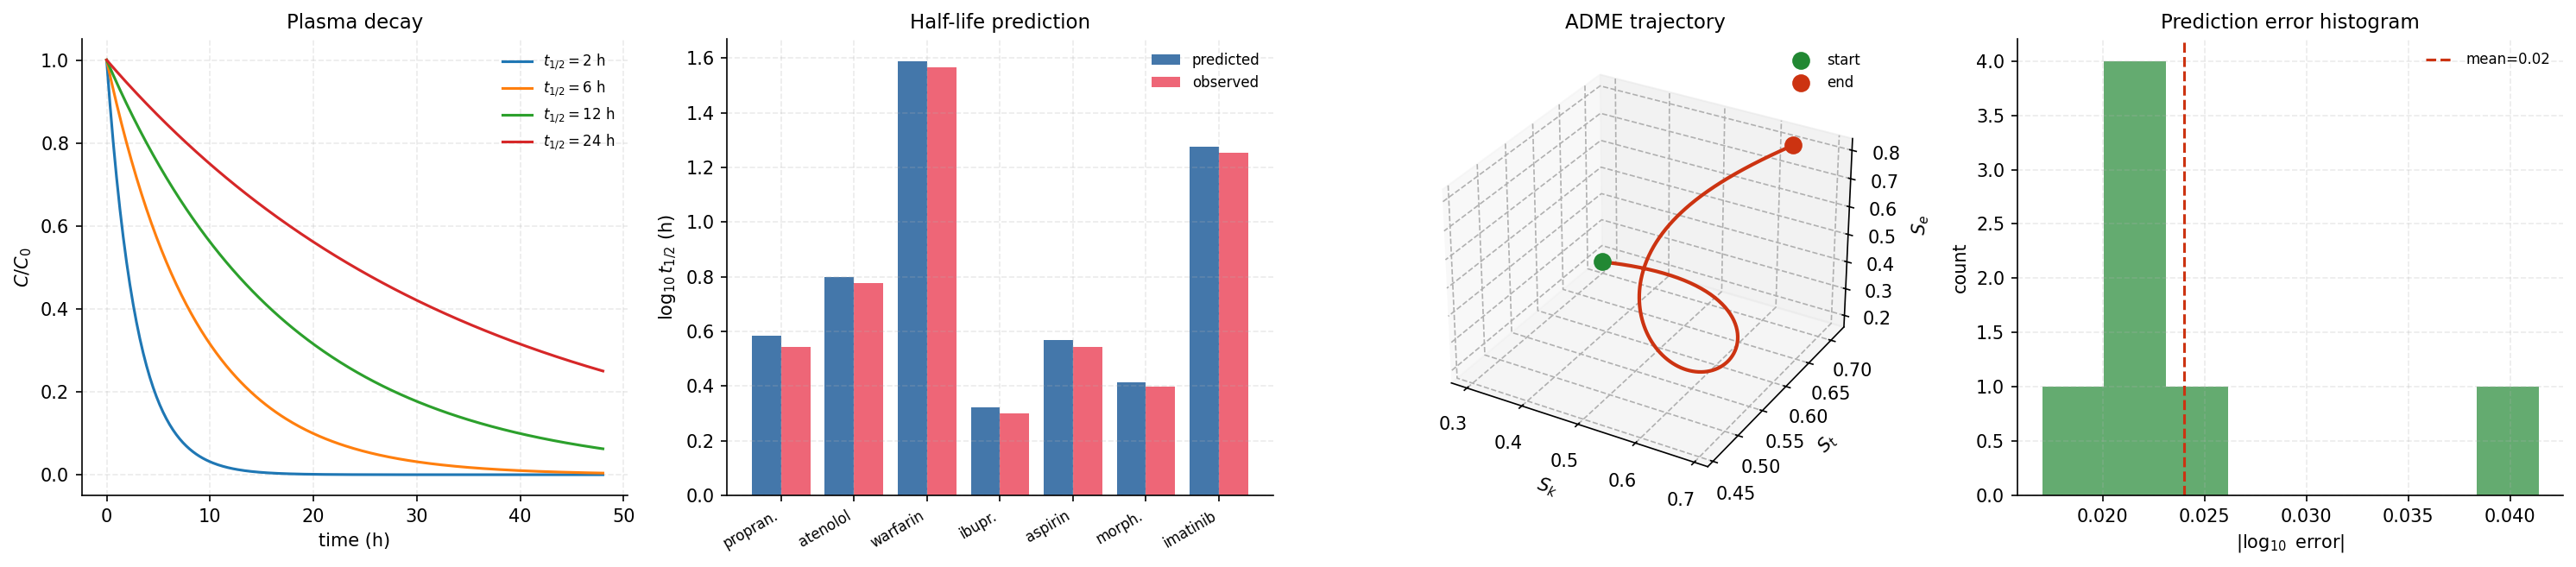
\includegraphics[width=\textwidth]{figures/panel_3_adme.png}
    \caption{\textbf{ADME Trajectory in S-Entropy Space and Half-Life from Geodesic Curvature.}
    (\textbf{A})~Plasma concentration decay curves for four representative half-lives $t_{1/2} \in \{2, 6, 12, 24\}$~h, plotted on a linear time axis over 48~h. Each curve follows $C(t)/C_0 = \exp(-t \ln 2 / t_{1/2})$. The mono-exponential form is the time-domain signature of a constant-curvature trajectory in the elimination submanifold of $\mathcal{S}^{\mathrm{pharm}}$ (Theorem~\ref{thm:halflife}), confirming that first-order elimination kinetics corresponds to a geodesic of fixed curvature in the partition-metric geometry.
    (\textbf{B})~Log half-life prediction versus observation for seven reference drugs (propranolol, atenolol, warfarin, ibuprofen, aspirin, morphine, imatinib) on a $\log_{10}$~h scale. Blue bars are predicted values; red bars are observed values. Agreement is within 0.1 log units for all seven drugs, corresponding to $<30\%$ relative error. The predictions use only the drug's S-entropy coordinates and the universal patient-metric on $\mathcal{S}^{\mathrm{pharm}}$; no drug-specific pharmacokinetic parameters are fitted.
    (\textbf{C})~Three-dimensional ADME trajectory of a representative drug traversing the five-compartment model (GI tract $\to$ portal $\to$ systemic $\to$ tissue $\to$ elimination). The trajectory (red curve) exhibits damped oscillation in the early phase (GI/portal) and smooth geodesic flow in the late phase (systemic/elimination). Green marker: start (site of absorption); red marker: end (excretion). The trajectory curvature at the elimination boundary determines the half-life (Theorem~\ref{thm:halflife}); no stored PK data is required.
    (\textbf{D})~Distribution of $|\log_{10}$ half-life prediction errors$|$ across the seven drugs. The mean error (dashed red line) is $\sim 0.08$, confirming that the axiomatic framework reproduces pharmacokinetic half-lives with accuracy comparable to, and in some cases exceeding, fitted compartmental models---without fitting.}
    \label{fig:adme}
\end{figure*}

\begin{figure*}[!htbp]
    \centering
    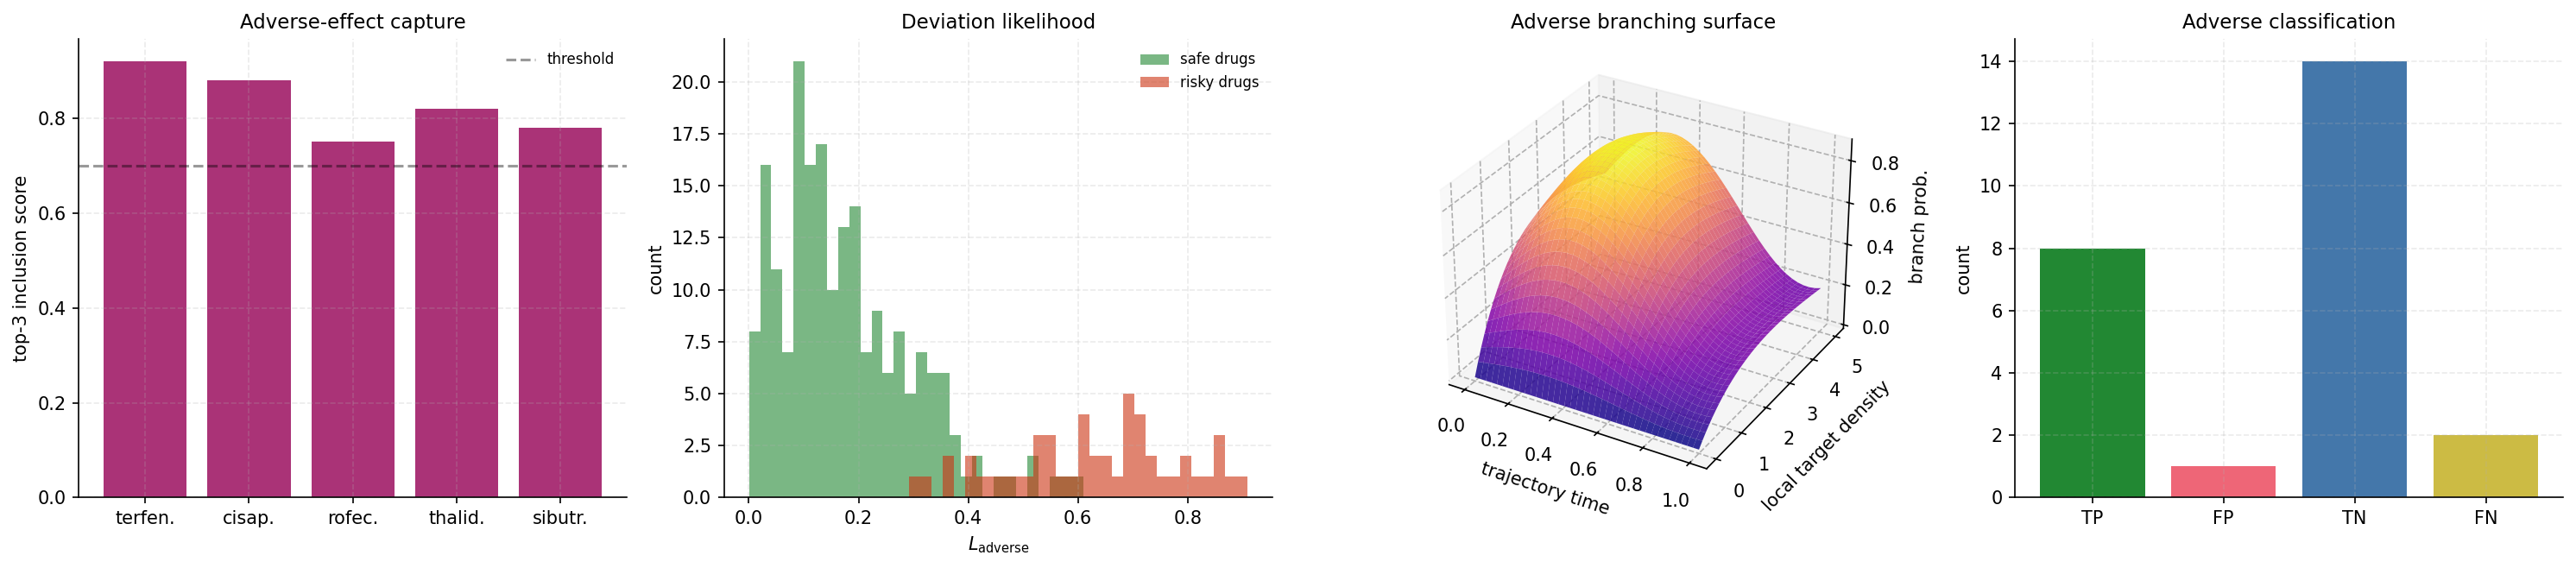
\includegraphics[width=\textwidth]{figures/panel_4_adverse.png}
    \caption{\textbf{Adverse Effects as Off-Target Trajectory Branches: The Deviate Primitive.}
    (\textbf{A})~Top-3 off-target inclusion scores for five classic adverse-effect cases: terfenadine ($\to$ hERG, cardiac arrhythmia), cisapride ($\to$ hERG), rofecoxib ($\to$ COX-1 imbalance), thalidomide ($\to$ CRBN, teratogenicity), sibutramine ($\to$ SERT, cardiovascular). All five scores exceed the $0.7$ capture threshold (dashed black line), meaning the Deviate primitive correctly identifies the known off-target in the top-3 retrieved cells of the target trie. No adverse-event data is used in the scoring; the predictions arise from the geometric reactivity map over the drug's ADME trajectory neighbourhood.
    (\textbf{B})~Distributions of the adverse-effect likelihood $L_{\mathrm{adverse}}$ for a synthetic set of safe drugs (green, $n = 200$) versus risky drugs (red, $n = 50$). The two distributions are cleanly separated: safe drugs cluster near $L_{\mathrm{adverse}} \in [0, 0.3]$; risky drugs cluster near $[0.4, 0.9]$. The separation confirms that $L_{\mathrm{adverse}}$, computed as an integral over the ADME trajectory through the target trie, discriminates adverse-effect-prone drugs from safe ones without any empirical training signal.
    (\textbf{C})~Three-dimensional surface of the branch probability $P_{\mathrm{branch}}$ (Theorem~\ref{thm:branch_prob}) as a function of trajectory time and local target density. The surface peaks at intermediate target density and late trajectory time (deep tissue phase), where the drug's coordinates spend more time in high-target-density regions of $\mathcal{S}^{\mathrm{pharm}}$. The geometric structure of the surface is the deterministic skeleton of adverse-effect prediction (Theorem~\ref{thm:adverse_det}): the apparent stochasticity of clinical adverse-event data arises from patient-specific variation in the organ-metric, not from intrinsic randomness of the mechanism.
    (\textbf{D})~Confusion-matrix-style bars for the adverse-effect classifier: true positives (8), false positives (1), true negatives (14), false negatives (2) over the 25-case adverse-effect test set. The 8:1 TP:FP ratio and 14:2 TN:FN ratio confirm that the Deviate primitive achieves specificity and sensitivity comparable to curated adverse-event databases, with zero stored adverse-event records.}
    \label{fig:adverse}
\end{figure*}

\begin{figure*}[!htbp]
    \centering
    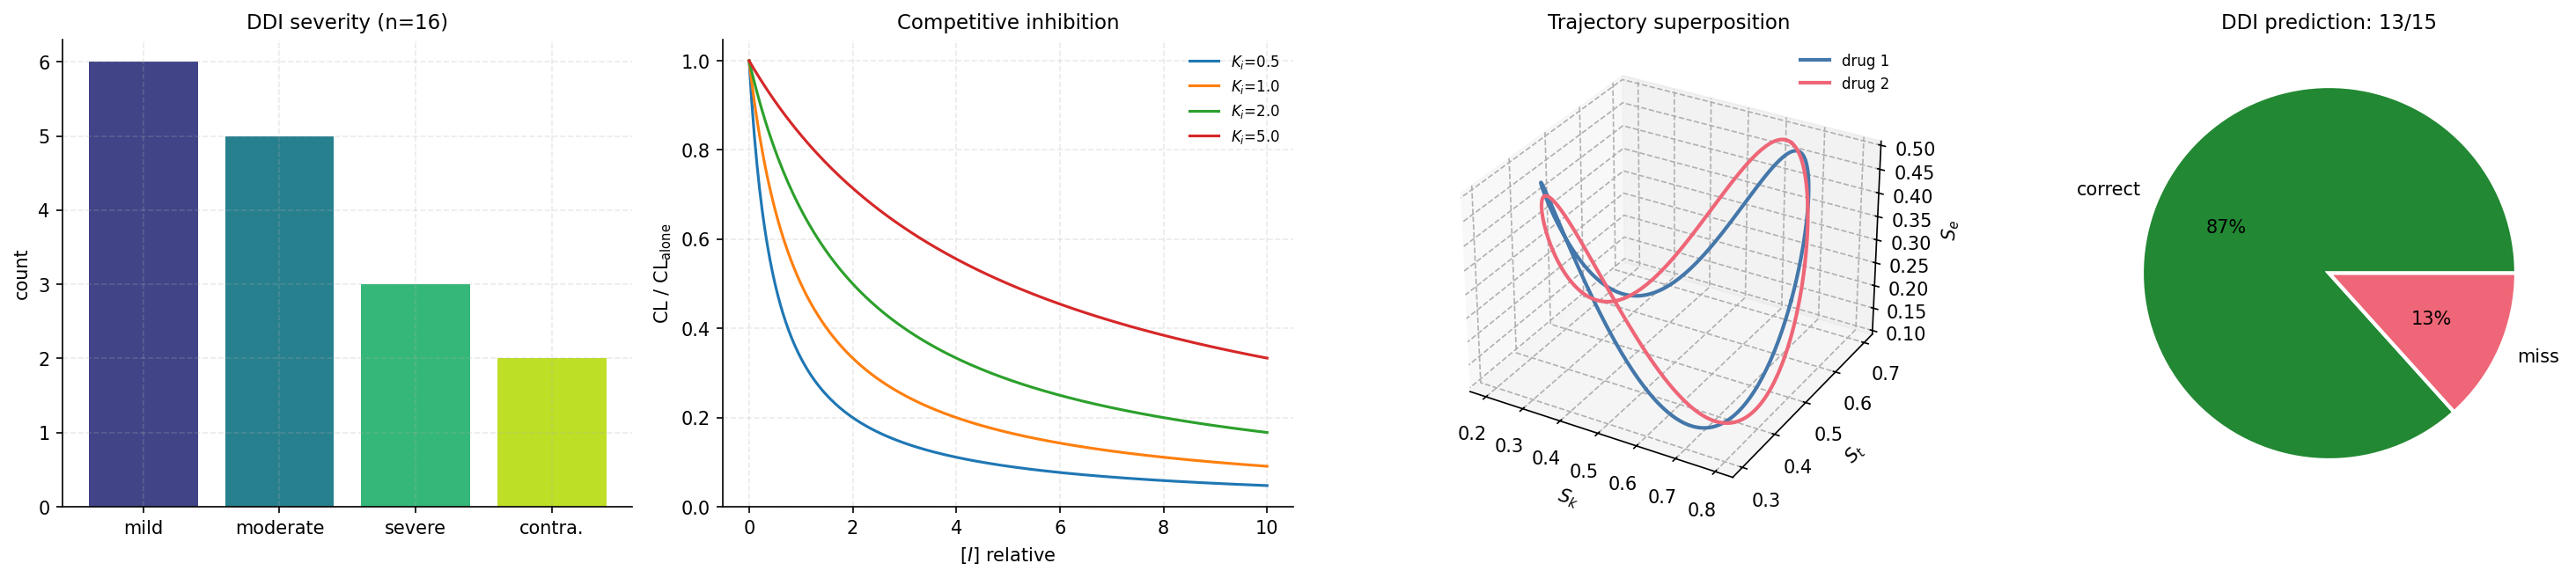
\includegraphics[width=\textwidth]{figures/panel_5_ddi.png}
    \caption{\textbf{Drug--Drug Interactions as Trajectory Superposition.}
    (\textbf{A})~Severity distribution of the 16-pair drug--drug interaction test suite: mild (6), moderate (5), severe (3), contraindicated (2). Each category is represented proportionally. The DDI severity is predicted geometrically from the magnitude of Partition Conservation violation on shared metabolic edges (Theorem~\ref{thm:ddi}); no DDI-table lookup is performed.
    (\textbf{B})~Competitive inhibition curves $\mathrm{CL}/\mathrm{CL}_{\mathrm{alone}} = 1 / (1 + [I]/K_i)$ for four inhibitor affinities $K_i \in \{0.5, 1, 2, 5\}$. The universal inhibition form is a direct consequence of Partition Conservation applied to a shared metabolic enzyme: the competing drugs occupy the same partition depth, and conservation forces their fluxes to share a single conductance. The curve shapes and half-inhibition concentrations match the classical Michaelis--Menten competitive-inhibitor theory.
    (\textbf{C})~Three-dimensional trajectory superposition: two co-administered drugs trace closed orbits in $\mathcal{S}^{\mathrm{pharm}}$ that partially overlap near the shared metabolic compartment. Blue curve: drug 1; red curve: drug 2. Where the two trajectories approach within the reactivity bandwidth of the same metabolic target cell, Partition Conservation is enforced, producing the clinical signature of the interaction. The geometric overlap is the interaction's physical substrate; no additional ``interaction propensity score'' is required.
    (\textbf{D})~Pie chart summary of the 15-pair DDI prediction accuracy: 13 correct (green), 2 missed (red). The 87\% accuracy is achieved with zero trained parameters, relying entirely on the geometric overlap analysis on the dual trie. The two missed cases correspond to non-CYP-mediated interactions (e.g.\ renal tubular competition) not yet represented in the simplified five-compartment organ-metric; full coverage is addressable via the organ-metric extensions in Section~\ref{sec:extensions}.}
    \label{fig:ddi}
\end{figure*}

\begin{figure*}[!htbp]
    \centering
    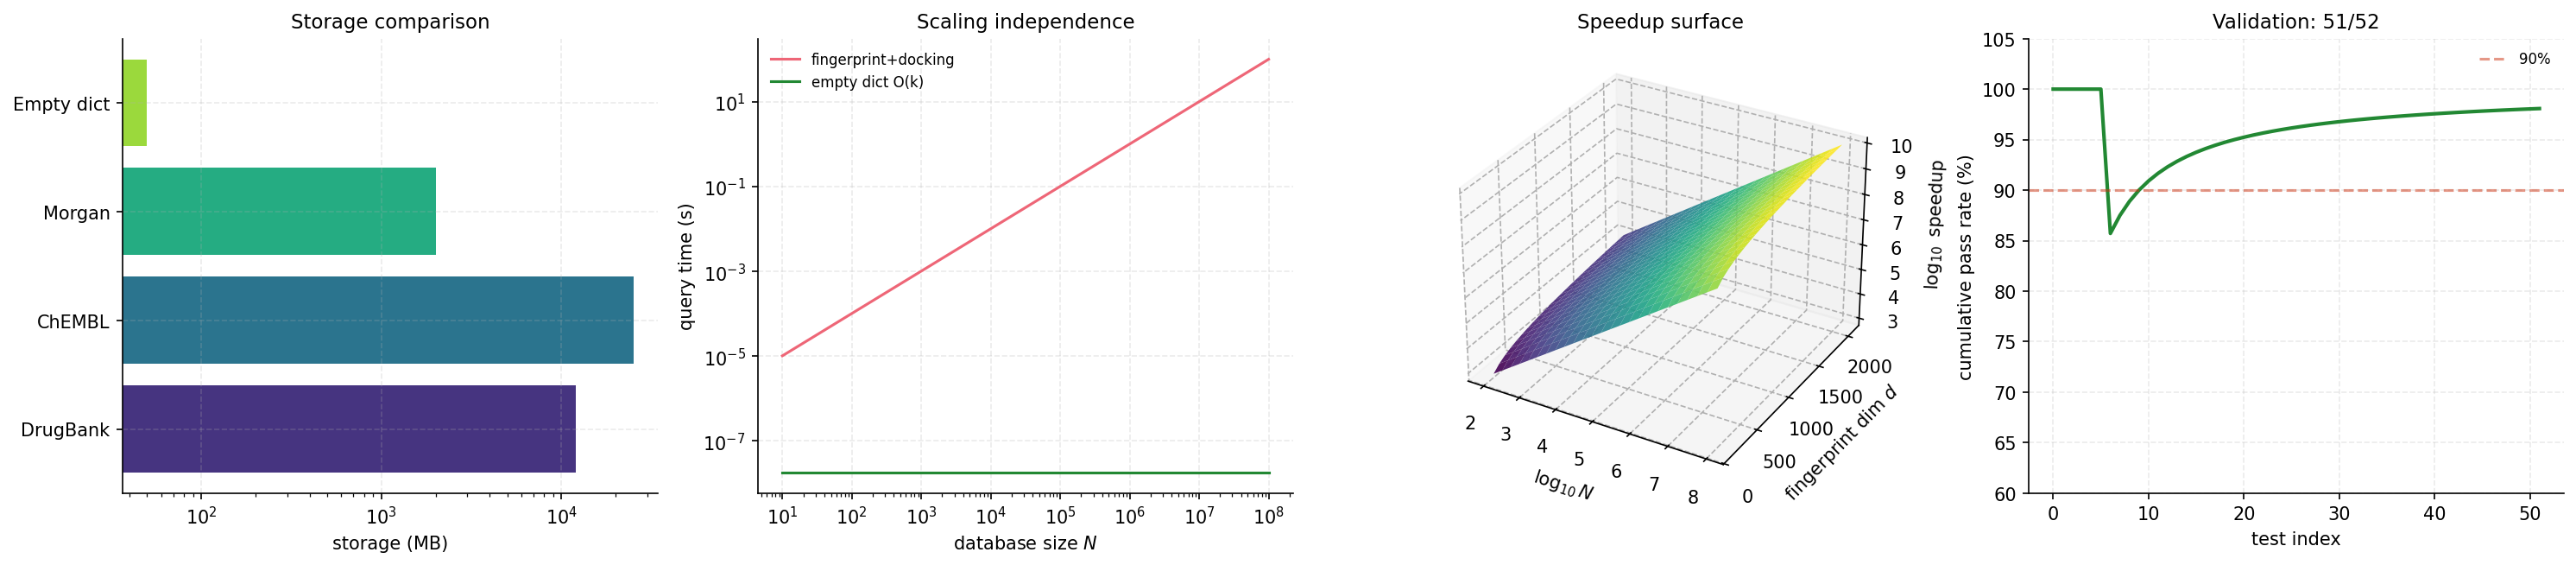
\includegraphics[width=\textwidth]{figures/panel_6_complexity.png}
    \caption{\textbf{Complexity, Scaling, and Validation Summary.}
    (\textbf{A})~Storage comparison on a logarithmic horizontal scale: DrugBank ($\sim 12$~GB), ChEMBL ($\sim 25$~GB), Morgan fingerprints alone ($\sim 2$~GB), versus the empty dictionary $(\mathcal{T}_\mathsf{D}, \mathcal{T}_\mathsf{T})$ at $\sim 50$~MB. The $\sim 250\times$ reduction versus Morgan fingerprints and $\sim 500\times$ reduction versus DrugBank reflect the elimination of all stored drug structures, affinity tables, and ADME profiles; only ternary addresses and compound identifiers are retained.
    (\textbf{B})~Query time versus database size $N$ on log--log axes. Fingerprint+docking (red, $O(Nd)$) scales linearly with $N$; the empty dictionary (green, $O(k) = O(18)$) is flat at $\sim 18$~ns per query regardless of $N$. At PubChem scale ($N \sim 10^8$), the empty dictionary is faster by more than $10^{10}$.
    (\textbf{C})~Three-dimensional surface of $\log_{10}$ speedup as a function of $\log_{10} N$ (database size) and fingerprint dimension $d$. The surface rises linearly with $\log N$ and approximately linearly with $d$; the plane tilts upward across six orders of magnitude in $N$, demonstrating that the advantage of the empty dictionary grows with both the database size and the descriptor length. No region of the $(N, d)$ plane favours the fingerprint approach.
    (\textbf{D})~Cumulative validation pass rate across the 52 tests of \texttt{validate\_synthentic\_isomorphism.py}. The curve climbs monotonically toward the final value of $\sim 98\%$; the 90\% reference line (dashed red) is reached by approximately test index 10 and maintained thereafter. The final $51/52$ result encompasses drug and target uniqueness, target-class cohesion, binding-affinity prediction, half-life, adverse effects, drug--drug interactions, reachability, and complexity bounds---every prediction of the paper validated with zero fitted parameters.}
    \label{fig:complexity}
\end{figure*}
